\documentclass[12pt]{article}

%%%%%%%%%%%%%%%%%
% the packages
\usepackage[utf8]{inputenc}
\usepackage[a4paper,margin=1in]{geometry}
\usepackage{graphicx,caption,subcaption}
\graphicspath{{./figures}}
\usepackage{color,hyperref}
\hypersetup{colorlinks=true,urlcolor=blue,citecolor=blue,linkcolor=blue}
\usepackage{enumitem}

\usepackage{multicol,longtable,multirow,booktabs,array}
\usepackage[authoryear]{natbib}
\bibliographystyle{plainnat}

\usepackage{mathaddons}

\newcommand{\sr}[1]{\textcolor{red}{#1}}


%%%%%%%%%%%%%%%%%%%%%%%%%
\title{Notes on High Dimension Probability}
\author{Subhrajyoty Roy}
\date{\today}


\begin{document}
\allowdisplaybreaks
\maketitle

\begin{abstract}
    This contains the lecture notes of the course on \textit{High Dimensional Probability} by Roman Vershynin. The course is available for free at online~\url{https://www.math.uci.edu/~rvershyn/teaching/hdp/hdp.html}.
\end{abstract}

\tableofcontents


\section{Introduction to High Dimensional Ideas}

\textbf{Big data} can come in one of two different ways.
\begin{enumerate}
    \item \# observations is big, this is usually easy, as classical statistical theory tells us how to deal with large number of samples. These are often better.
    \item \# dimensions is big. This is usually hard.
\end{enumerate}

Empirical observation: it is exponentially harder to deal with larger \# of dimensions rather than larger \# of observations. To illustrate this, let's consider an example problem.

\begin{example}
    Let's say we want to numerically compute the integral
    \begin{equation*}
        \int_0^1 \cdots \int_0^1 f(x_1, \ldots, x_d) dx_1 \ldots dx_d
    \end{equation*}
    The usual way is to perform a numerical integration approach, based on Riemann sums. For $d = 1$, we can subdivide the interval $[0, 1]$ into grids of width (or resolution) $\epsilon$, so there are $1/\epsilon$-grids. Then, we have the Riemann sum as
    \begin{equation*}
        \int_{[0, 1]} f(x)dx \approx \dfrac{1}{n}\sum_{i=1}^n f(x_i), \ n = (1/\epsilon).
    \end{equation*}
    \noindent Note that, this will ensure that the bias is of order $O(\epsilon)$, assuming $f$ is bounded. To see this,
    \begin{align*}
        \left\vert \int_{[0, 1]} f(x)dx - \dfrac{1}{n}\sum_{i=1}^n f(x_i) \right\vert
         & \leq \dfrac{1}{n}\sum_{i=1}^{n} \left\vert \int_{[(i-1)/n, i/n]} f(x)dx - f(x_i) \right\vert \\
         & = \dfrac{1}{n}\sum_{i=1}^{n} \left\vert f(t_i) - f(x_i) \right\vert                          \\
         & = O(1/n) = O(\epsilon)
    \end{align*}
    \noindent where $t_i$ is a tag obtained by using Integral Mean Value Theorem on $f$, for the interval $[(i-1)/n, i/n]$.

    In general, for $d$-dimensional hypercube $[0, 1]^d$, we require $n = O(1/\epsilon^d)$ many points to achieve an error bound of $O(\epsilon)$.
\end{example}

Therefore, we need the number of points to be exponential in dimension to achieve the same level of accuracy. This is also called \textbf{the curse of dimensionality}.

However, there is a better way to solve this problem, by using Monte Carlo method, which uses probabily to achieve good result for this. Instead of choosing the points on the grid, choose uniformly at random. Pick $N$ points:

\begin{equation*}
    S_N = \dfrac{1}{N}\sum_{i=1}^N f(x_i), \ x_i \sim \text{Uniform}([0, 1]^d)
\end{equation*}

Note that, $\E(S_N) = \E(f(X)) = \int_{[0, 1]^d} f(x)dx$. The average $L^2$ error is given by
\begin{align*}
    \E\left[\left(\frac{1}{N} \sum_{i=1}^N f(x_i) - \int_{[0,1]^d} f(x) dx\right)^2 \right]
     & = \var\left( \frac{1}{N} \sum_{i=1}^N f(x_i) \right) \\
     & = \dfrac{\var(f(X))}{N} \leq C/N
\end{align*}
\noindent since $f(x)$ is bounded. Therefore, the RMSE = $O(\frac{1}{\sqrt{N}})$, independent of the dimension $d$.

\begin{note}
    Thinking in terms of probability might help to overcome in high-dimensional inference problems.
\end{note}


\subsection{Convexity}

Usually in high-dimensional (HD) problems, convexity helps a lot.

\begin{definitionbox}
    A set $T \subset \R^n$ is convex if $\forall x,y \in T$, the segment $[x,y] \in T$.
\end{definitionbox}

Let us consider a few examples as follows:

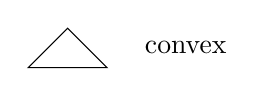
\begin{tikzpicture}[scale=0.5]
    \draw (0,0) -- (1,1) -- (2,0) -- cycle;
    \node at (4,0.5) {convex};
\end{tikzpicture}


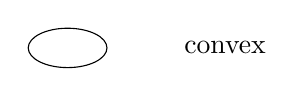
\begin{tikzpicture}[scale=0.5]
    \draw (3,0) ellipse (1cm and 0.5cm);
    \node at (7, 0) {convex};
\end{tikzpicture}


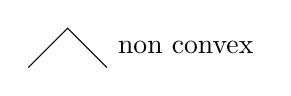
\begin{tikzpicture}[scale=0.5]
    \draw (6,0) -- (7,1) -- (8,0);
    \node at (10,0.5) {non convex};
\end{tikzpicture}


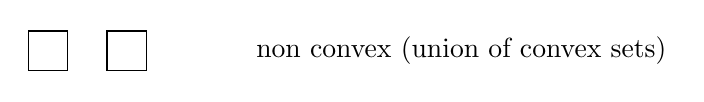
\begin{tikzpicture}[scale=0.5]
    \draw (9,0) rectangle (10,1);
    \draw (11,0) rectangle (12,1);
    \node at (20,0.5) {non convex (union of convex sets)};
\end{tikzpicture}

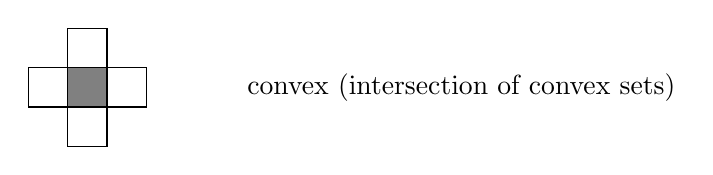
\begin{tikzpicture}[scale=0.5]
    \draw (5,0) rectangle (8,1);
    \draw (6,-1) rectangle (7,2);
    \draw[fill = gray] (6,0) rectangle (7,1);
    \node at (16,0.5) {convex (intersection of convex sets)};
\end{tikzpicture}

This means union of convex sets may not be convex, but intersection of convex sets is convex. Thus, starting with a set $T$, we can consider the intersection of all such convex sets that are superset of $T$.

\begin{definitionbox}
    The convex hull $\text{conv}(T)$ of a set $T \subset \R^n$ is the smallest convex set that contains $T$.
\end{definitionbox}

\begin{theorembox}
    $\forall z \in \text{conv}(T)$, we have a decomposition, $z = \sum_{i=1}^m \lambda_i z_i$, where, $\lambda_i \geq 0$, $\sum_{i=1}^m \lambda_i = 1$, and each $z_i \in T$. Note that, the above combination or representation may not be unique or parsimonious.
\end{theorembox}

\begin{theorembox}[Caratheodory Theorem]
    $\forall z \in \text{conv}(T)$, $\exists$ a representation (convex combination) of $\leq (n+1)$ points in $T$, where, $T \subset \R^n$.
\end{theorembox}

Note that, the choice of basis in the representation obtained by the Caratheodory Theorem may depend on the choice of $z$. Also, the number $(n+1)$ is unimprovable, there is a dimension dependence here. However, it turns out that if we allow to get $z$ back only approximately, we can use a similar trick like the Monte Carlo method to get a better representation, that may be dimension-independent. Additionally it says that we can choose the weights to be the same, and still get a good approximate solution.

\begin{theorembox}[Approximate Caratheodory Theorem]
    Let $T \subset \R^n$, and $\text{diam}(T) \leq 1$ (otherwise we can rescale). Then, $\forall z \in \text{conv}(T)$, $\forall k \in \N$, $\exists z_1, z_2, \ldots, z_k \in T$ (these points may be same) such that
    \begin{equation*}
        \left\Vert z - \frac{1}{k} \sum_{i=1}^k z_i\right\Vert_2 \leq \frac{1}{\sqrt{2k}}
    \end{equation*}
    This means, if we want error to be less than equal to $\epsilon$, the choose, $k = \frac{1}{2\epsilon^2}$ (which is dimension free).
\end{theorembox}

\begin{proof}
    \textbf{This proof is also called Empirical Method of Maurey}.

    Fix any $z \in \text{conv}(T)$, by Caratheory Theorem, we have, $z = \sum_{i=1}^m \lambda_i z_i$, $\lambda_i \geq 0$, $\sum_{i=1}^m \lambda_i = 1$, $z_i \in T$.

    Now, consider a random variable (r.v.) $Z$ that takes value $z_i$, with probability $\lambda_i$. Then, $\E(Z) = \sum_{i=1}^m \lambda_i z_i = x$. Let, $X_1, X_2, \dots X_k \equiv Z$ be iid copies of $Z$. Therefore, the $L^2$ error is
    \begin{align*}
        \E\left(\left\Vert z - \frac{1}{k} \sum_{i=1}^k X_i\right\Vert_2^2\right)
         & = \E\left\Vert \frac{1}{k} \sum_{i=1}^k (X_i - z)\right\Vert_2^2                                           \\
         & = \frac{1}{k^2} \sum_{i=1}^k \E\left\Vert X_i - \E(X_i)\right\Vert_2^2, \text{ since } z = \E(Z) = \E(X_i) \\
         & = \frac{1}{k} \E\left\Vert Z - \E(Z)\right\Vert_2^2, \text{ since } X_i \equiv Z                           \\
         & = \frac{1}{2k} \E\left\Vert Z - Z'\right\Vert_2^2, \text{ where } Z' \text{ is an independent copy of } Z  \\
         & \leq \frac{1}{2k}, \text{ as } \left\Vert Z-Z'\right\Vert_2^2 \leq \text{diam}(T) \leq 1
    \end{align*}

    \noindent So since, the expectation $\leq \frac{1}{2k} \Rightarrow \exists$ a realization of $X_i$'s such that $L^2$ error $\leq \frac{1}{2k}$. Therefore, $\left\Vert z - \frac{1}{k} \sum_{i=1}^k z_i\right\Vert_2^2 \leq \frac{1}{2k}$, where, $z_i$'s are the realizations of $X_i$, and hence each $z_i \in T$.
\end{proof}

\begin{exercisebox}
    Let $x_1, x_2, \dots x_n$ be an arbitrary set of unit vectors in $\R^n$. Prove that there exists $\epsilon_1, \epsilon_2, \dots, \epsilon_n$ with $\epsilon_i \in \{-1, +1\}$ such that $\Vert \sum_{i=1}^n \epsilon_i x_i\Vert_2 \leq \sqrt{n}$.

    To solve this, we use probabilistic methods. Note that, if $\epsilon_i$s are random variables, then the expected squared $L^2$ norm is
    \begin{equation*}
        \E\Vert \sum_{i=1}^n \epsilon_i x_i\Vert_2^2 = \sum_{i=1}^n \Vert x_i\Vert^2 \E(\epsilon_i^2) = n
    \end{equation*}
    \noindent since $x_i$ is unit vector and $\E(\epsilon_i^2) = \var(\epsilon_i) + \E^2(\epsilon_i) = 1$. This means, there exists a realization that has squared $L^2$ norm less than equal to $n$, i.e., the $L^2$ norm less than equal to $\sqrt{n}$.
\end{exercisebox}

\subsection{Applications of ACT}

There are multiple applications of ACT. One useful idea is in portfolio building, where the ingredients are ``stocks'', and their linear combination is basically a mutual fund. The problem is to create a new mutual fund with a given combination of stocks by mixing available mutual funds, (i.e., the fund of funds). The solution is to use ACT to obtain a fast randomized solution approximately.

\begin{note}
    Note that, ACT only provides the existence, and does not necessarily provide an algorithm to find that out. However, one simple algorithm could be to start with all the available mutual funds and then take any $k$ of them randomly and average their returns.
\end{note}

Another prominent application of ACT is in covering numbers. This is what we will explore now.

\begin{definitionbox}
    The \textbf{Covering Number} of a set $T \subset \mathbb{R}^n$ at scale $\epsilon > 0$ is the smallest \# of Euclidean balls of radius $\epsilon$ needed to cover $T$. It is denoted by $N(T,\epsilon)$.
\end{definitionbox}

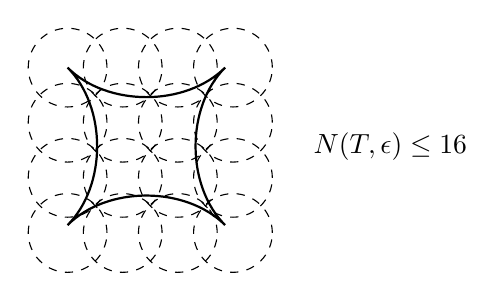
\begin{tikzpicture}
    % Draw the concave shape with four corners
    \draw[thick] (0,0) .. controls (0.5,-0.5) and (1.5,-0.5) .. (2,0)
    .. controls (1.5,-0.5) and (1.5,-1.5) .. (2,-2)
    .. controls (1.5,-1.5) and (0.5,-1.5) .. (0,-2)
    .. controls (0.5,-1.5) and (0.5,-0.5) .. (0,0);

    % Draw unit circles covering the shape
    \foreach \x in {0, 0.7, 1.4, 2.1} {
            \foreach \y in {0, -0.7, -1.4, -2.1} {
                    \draw[dashed, fill=none] (\x,\y) circle (0.5);
                }
        }
    \node[right] at (3,-1) {$N(T,\epsilon) \leq 16$};
\end{tikzpicture}

\begin{lemmabox}
    Let $B$ be the unit Euclidean ball, then we have $N(B, \frac{1}{2}) \geq 2^d$, i.e., the covering number is exponential in dimension.
\end{lemmabox}

\begin{proof}
    Assume $B$ can be covered by $N$ copies of $(\frac{1}{2}B)$ ball. Then clearly,
    \begin{align*}
                 & Vol(B) \leq N \cdot Vol\left(\frac{1}{2}B\right), \text{ since RHS might have some overlaps.} \\
        \implies & Vol(B) \leq N 2^{-d} Vol(B)                                                                   \\
        \implies & N \geq 2^d
    \end{align*}
\end{proof}

This is an unsurprising result. However, what is surprising is that the covering number for a polytope (i.e., a higher dimensional analogue of polygon), is independent of the dimension but dependent only on the number of vertices. Also, it is polynomial in the number of vertices.

\begin{lemmabox}
    Let $P$ be a polytope in $\R^d$ with $m$ vertices and $\text{diam}(P) \leq 1$. Then, $N(P, \epsilon) \leq m^{1/2\epsilon^2}$.
\end{lemmabox}
\begin{proof}
    If we consider, $P$ to be nonconvex, then $conv(P)$ is a polytope with $\leq m$ vertices. This can only weaken the bound. Therefore, it is enough to show it for the cases when $P$ is convex.

    Let $T$ be the set of vertices of $P$. Clearly, $P \subseteq conv(T)$. Note that ACT implies that $\forall z \in P$, is within distance $\frac{1}{\sqrt{2k}}$ from some point in the set
    \begin{equation*}
        \mathcal{N} := \left\{\frac{1}{k} \sum_{i=1}^k z_i : z_i \in T \right\}.
    \end{equation*}
    \noindent This means, $\forall x \in P$, is covered by a ball of radius $\frac{1}{\sqrt{2k}}$ and center $\in \mathcal{N}$. This means, the covering number
    \begin{equation*}
        N(P, 1/\sqrt{2k}) \leq \vert \mathcal{N}\vert \leq m^k,
    \end{equation*}
    \noindent since to choose an element of $\mathcal{N}$, we pick any $k$ vertices from $m$ vertices which is $\binom{m}{k} = O(m^k)$. Choosing $\epsilon = 1/\sqrt{2k}$ now completes the proof.
\end{proof}

To make use of these results, usually, it helps by considering the intuition that, a small covering \# $\Rightarrow$ small volume, $\Rightarrow$ easier to apply union-type bounds. As a result, since the covering number of a polytope is small, we expect the volume of the polytope also be to small compared to the Euclidean ball.

\begin{theorembox}[Carl-Pajor, 88]
    Let $B$ be the unit Euclidean ball, and $P \subset B$ be any polytope with $m$ vertices in $\R^n$. Then,
    \begin{equation*}
        \dfrac{Vol(P)}{Vol(B)} \leq \left( 4\dfrac{\sqrt{\log m}}{\sqrt{n}} \right)^n
    \end{equation*}
\end{theorembox}
\noindent What the Carl-Pajor theorem tells us is that the volume of the polytope is extremely small, unless the number of vertices $m$ is exponential in $n$.

\begin{proof}
    Let us consider $\epsilon B$-balls and cover $P$ with these balls. By definition of covering number, we have
    \begin{align*}
                 & Vol(P) \leq N(P,\epsilon) Vol(\epsilon B)                                   \\
        \implies & Vol(P) \leq N(P, \epsilon) \epsilon^n Vol(B)                                \\
        \implies & Vol(P)/Vol(B) \leq \epsilon N(P, \epsilon) \leq \epsilon^n m^{2/\epsilon^2}
    \end{align*}
    \noindent Here, we use the previous Lemma, but with the understanding that since $B$ is a unit Euclidean ball, its diameter is $2$. Now, note that the above inequality is true for every $\epsilon > 0$. Therefore,
    \begin{equation*}
        \frac{Vol(P)}{Vol(B)} \leq \inf_{\epsilon > 0} \epsilon^n \cdot m^{\frac{1}{2\epsilon^2}}.
    \end{equation*}
    \noindent Let $\ell(\epsilon) = \epsilon^n m^{\frac{1}{2\epsilon^2}} \Rightarrow \log \ell(\epsilon) = n \log \epsilon + \frac{1}{2\epsilon^2} \log m$. Now setting its derivative equal to $0$, we get $\frac{\partial \log l}{\partial \epsilon} = 0 = \frac{n}{\epsilon} - \frac{1}{\epsilon^3} \log m \Rightarrow \epsilon = \sqrt{\frac{4 \log m}{n}}$. Putting this value of $\epsilon$ based into the expression, we get
    \begin{align*}
        \inf_{\epsilon > 0} \ell(\epsilon)
         & = \exp\left[ n \log\left( \dfrac{\sqrt{4\log m}}{\sqrt{n}} \right) + \dfrac{2\log m}{4\log m} n \right] \\
         & = \exp\left[ \log\left( \dfrac{\sqrt{4\log m}}{\sqrt{n}} \right)^n e^{n/2} \right]                      \\
         & = \left( \dfrac{\sqrt{4e \log m}}{\sqrt{n}} \right)^n
        \leq \left( 4\dfrac{\sqrt{\log m}}{\sqrt{n}} \right)^n, \text{ since } e \leq 4.
    \end{align*}
\end{proof}

A few remarks we want to make here.
\begin{itemize}
    \item Carl-Pajor proved a slightly better result, with $\log(m/n)$ rate, which is optimal.
    \item The optimal bound is attained at a random polytope. (Dafnis et al., 2003, 2009)
    \item Let $\delta = 4\sqrt{\frac{\log m}{n}}$, then note that, $Vol(\delta B) = \delta^n \cdot Vol(B)$, and correspondingly, $\Rightarrow \frac{Vol(\delta B)}{Vol(B)} = \delta^n \geq \frac{Vol(P)}{Vol(B)}$. As a result, we have $Vol(\delta B) \geq Vol(P)$. This means, a small ball around origin has at least the same volume as the polytope.
\end{itemize}

This means, the low-dimensional picture that we usually think is wrong.

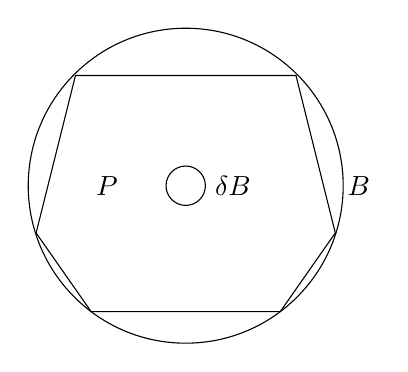
\begin{tikzpicture}
    \draw (0,0) circle (2cm);
    \draw (0,0) circle (0.25cm);
    \draw (-1.9,-0.6) -- (-1.4,1.4) -- (1.4,1.4) -- (1.9,-0.6) -- (1.2, -1.6) -- (-1.2, -1.6) -- cycle;
    \node at (-1,0) {$P$};
    \node at (0.6,0) {$\delta B$};
    \node at (2.2,0) {$B$};
\end{tikzpicture}

\noindent For correct intuition in high dimension, we can consider the hyperbolic correction by ``V. Milman''.

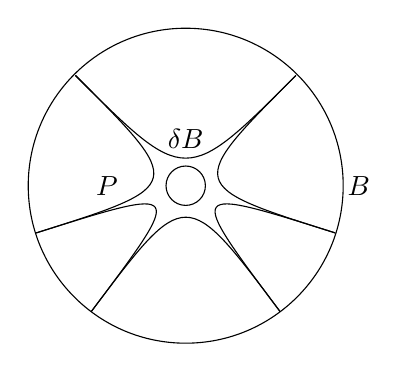
\begin{tikzpicture}
    \draw (0,0) circle (2cm);
    \draw (0,0) circle (0.25cm);
    \draw (-1.9, -0.6) .. controls (0, 0) .. (-1.4, 1.4);
    \draw (-1.4, 1.4) .. controls (0, 0) .. (1.4, 1.4);
    \draw (1.4, 1.4) .. controls (0, 0) .. (1.9, -0.6);
    \draw (1.2, -1.6) .. controls (0, 0) .. (1.9, -0.6);
    \draw (1.2, -1.6) .. controls (0, 0) .. (-1.2, -1.6);
    \draw (-1.9, -0.6) .. controls (0, 0) .. (-1.2, -1.6);
    \node at (-1,0) {$P$};
    \node at (0,0.6) {$\delta B$};
    \node at (2.2,0) {$B$};
\end{tikzpicture}

\noindent The part $\delta B$ is called the ``core'' of the polytope. Note that, the polytope is convex, but it does not look convex. This is because, for high dimensional inference, we cannot completely visualize all the information. So here, we drop the convexity (because we can work with it algebraically), and instead work with the volume-based ideas (because probabilities map to volume in terms of measures).


\pagebreak
\section{Concentration Inequalities}

We know by law of large numbers that i.i.d. sum of a random variable $\bb{X}$ converges to $\E(X)$. The central limit theorem also tells that the rate of this convergence is $1/\sqrt{n}$. Since the central limit theorem and law of large numbers are very universal in nature, one might want to know to what extent these kinds of concentration holds. The fundamental aim of concentration inequalities is to demonstrate that a random variable (or i.i.d. sum of it) satisfies $X \approx \E(X)$ with high probability (exponentially close to $1$).

For example, in case of normal distribution, $X \sim N(\mu, \sigma^2)$, we know that
\begin{equation*}
    \prob(\vert X - \mu\vert > 3\sigma) = 0.9973.
\end{equation*}

For general distribution, we have
\begin{align*}
    \prob(X \geq t)                 & \leq \dfrac{\E(X)}{t}, \ \forall t > 0, \ \text{(because of Markov's inequality)}       \\
    \prob(\vert X - \E(X)\vert > t) & \leq \dfrac{\sigma^2}{t^2}, \ \forall t > 0, \ \text{because of Chebyshev's inequality}
\end{align*}

However, for Gaussian distribution, the concentration around the mean is much faster. To see this, consider the following Lemma.

\begin{theorembox}
    Suppose $g \sim N(0, 1)$, then
    \begin{equation*}
        \prob(g > t) \leq \frac{1}{\sqrt{2\pi}} \frac{e^{-t^2/2}}{t},
    \end{equation*}
    \noindent i.e., the tail probability decays exponentially fast in $t$.
\end{theorembox}
\begin{proof}
    \begin{align*}
        \prob(g > t) & = \int_{t}^{\infty} \frac{1}{\sqrt{2\pi}} e^{-x^2/2}dx                                               \\
                     & = \int_{0}^{\infty} \frac{1}{\sqrt{2\pi}} e^{-(t+y)^2/2} dy, \text{ using substitution } x = y + t   \\
                     & = \int_{0}^{\infty} \frac{1}{\sqrt{2\pi}} e^{-t^2/2} e^{-ty} e^{-y^2/2} dy                           \\
                     & \leq \int_{0}^{\infty} \frac{1}{\sqrt{2\pi}} e^{-t^2/2} e^{-ty} dy, \text{ since } e^{-y^2/2} \leq 1 \\
                     & = \frac{1}{\sqrt{2\pi}} e^{-t^2/2} \int_{0}^{\infty} e^{-ty} dy                                      \\
                     & = \dfrac{1}{\sqrt{2\pi} t} e^{-t^2/2}
    \end{align*}
\end{proof}

By symmetry, then we have for general $X \sim N(\mu, \sigma^2)$,
\begin{equation*}
    \prob(\vert X -\mu \vert > t\sigma) \leq \dfrac{1}{t}\sqrt{\dfrac{2}{\pi}} e^{-t^2/2} \leq e^{-t^2/2}, \text{ when } t \geq 1.
\end{equation*}

Therefore, the normal distribution has exponential tails.  Also, the central limit theorem (CLT) tells that
\begin{equation*}
    \sqrt{n} \left(\frac{\bar{X} - \mu}{\sigma}\right) \xrightarrow{d} Z \sim N(0,1),
\end{equation*}
\noindent so may be the tail probabilities are also close and exponential. But this does not work as the error from the CLT itself is of order $O(1/\sqrt{n})$, which is due to Berry-Esseen bound. So, the tail of $\sqrt{n} \left(\frac{\bar{X} - \mu}{\sigma}\right)$ does exponentially decay in general like Gaussian, at least by this route.

\begin{theorembox}[Berry Essen Bound]
    Let $X_i$ be i.i.d. random variables with mean $0$ and variance $1$, and finite third order moment. Then,
    \begin{equation*}
        \left\vert \prob\left( \dfrac{1}{\sqrt{N}}\sum_{i=1}^N X_i \geq t \right) - \prob(Z \geq t) \right\vert \leq \dfrac{\E(\vert X_1\vert^3}{\sqrt{N}} = O(1/\sqrt{N}),
    \end{equation*}
    \noindent where $Z \sim N(0, 1)$.
\end{theorembox}

\noindent So we would like to sidestep this CLT and try to control the tail of this normalized sum directly. This introduces the study of concentration inequalities.

\begin{exercisebox}
    Let $X$ be a standard normal random vector in $\R^n$ where $n \geq C_1$ (large constant). What are the values of $\E\Vert X\Vert_2^2$ and $\var(\Vert X\Vert_2^2)$?

    To obtain this, let $X_1, X_2, \dots X_n$ be the coordinates of the vector, note that
    \begin{align*}
        \E\Vert X\Vert_2^2     & = \E(X_1^2 + X_2^2 + \dots + X_n^2) = n \E(X_1^2) = n                                       \\
        \var(\Vert X\Vert_2^2) & = \var(X_1^2 + \dots + X_n^2) = n\var(X_1^2) = n\left[ \E(X_1^4) - \E^2(X_1^2) \right] = 2n
    \end{align*}
\end{exercisebox}

\begin{exercisebox}[Continued]
    Show that, $\vert \Vert X\Vert_2^2 - n\vert \leq C \sqrt{n}$ for some large $C$ with high probability (say $0.99$).

    To show this, we make use of Chebyshev's inequality. Note that,
    \begin{equation*}
        \prob(\vert \Vert X\Vert_2^2 - n\vert > t) = \prob(\vert \Vert X\Vert_2^2 - \E(\Vert X\Vert_2^2) \vert > t) \leq \dfrac{\var(\Vert X\Vert_2^2)}{t^2} = \dfrac{2n}{t^2}
    \end{equation*}
    \noindent Choosing $t = C\sqrt{n}$ for large $C$ yields, $\prob(\vert \Vert X\Vert_2^2 - n\vert > C\sqrt{n}) \leq 2/C$, which can be made smaller than $0.01$ by choosing large $C$.
\end{exercisebox}

\begin{exercisebox}[Continued]
    Deduce that this means, $\sqrt{n}/2 \leq \Vert X\Vert_2 \leq 2\sqrt{n}$ with high probability say $0.99$.

    Note that,
    \begin{equation*}
        \vert \Vert X\Vert_2 - \sqrt{n} \vert = \dfrac{\vert \Vert X\Vert_2^2 - n \vert}{\vert \Vert X\Vert_2 + \sqrt{n} \vert} = \dfrac{\leq C\sqrt{n}}{\geq \sqrt{n}} \leq C
    \end{equation*}
    \noindent with high probability. This says that for a random normal vector $X$, $\Vert X\Vert_2 = \sqrt{n} + o(1)$.
\end{exercisebox}

\begin{exercisebox}
    Let $X$ and $Y$ be two independent standard normal random vectors in $\R^n$ for some $n \geq C$. Find $\E\inner{X,Y}^2$ and $\var\inner{X,Y}^2$.

    Note that,
    \begin{align*}
        \E\inner{X,Y}^2
         & = \E\left( (\sum_{i=1}^n X_i Y_i)^2 \right)                                    \\
         & = \E\left[ \sum_{i=1}^n X_i^2 Y_i^2 + \sum_{i \neq j} X_iX_jY_iY_j \right] = n
    \end{align*}
    \noindent since $\E(X_i^2Y_i^2) = \E(X_i^2)\E(Y_i^2)$, by independence, and the second term is zero.

    Similarly,
    \begin{align*}
        \E\inner{X,Y}^4
         & = \E\left[ \left( \sum_{i=1}^n X_iY_i \right)^4 \right]                                                             \\
         & = \E\left[ \sum_{i=1}^n X_i^4 Y_i^4 + \sum_{i \neq j} X_i^2 Y_i^2 X_j^2 Y_j^2 \right], \text{ other terms are zero} \\
         & = n \times 3 \times 3 + n(n-1) \times 1 = n^2 + 8n
    \end{align*}
    \noindent Therefore, $\var\inner{X,Y}^2 = \E\inner{X,Y}^4 - \E^2\inner{X,Y}^2 = n^2 + 8n - n^2 = 8n$.
\end{exercisebox}

\begin{exercisebox}[(Continued)]
    Show that if the angle between those vectors is denoted by $\theta$, then $\vert \theta - \pi/2\vert = O(1/\sqrt{n})$ with large probability.

    We start by applying Chebyshev's inequality on $\inner{X,Y}^2$. Note that,
    \begin{equation*}
        \prob\left( \vert \inner{X,Y}^2 - n\vert \geq 3n \right) \leq \dfrac{\var\inner{X,Y}^2}{9n^2} = \dfrac{8}{9n} \rightarrow 0
    \end{equation*}
    \noindent Therefore, with sufficiently large probability, $\inner{X,Y}^2 \leq 4n$. This means,
    \begin{equation*}
        \cos^2(\theta) = \dfrac{\inner{X,Y}^2}{\norm{X}_2^2 \norm{Y}_2^2} = \dfrac{\leq 4n}{\geq (\sqrt{n} + o(1))^4} \leq \dfrac{C_2}{n}
    \end{equation*}
    \noindent i.e., $\vert \cos(\theta)\vert = O(1/\sqrt{n})$. Here we apply the result from previous exercise that $\norm{X}_2^2 = (\sqrt{n}+o(1))$. Therefore, $\vert \theta - \pi/2\vert = O(1/\sqrt{n}) \rightarrow 0$ as $n \rightarrow \infty$.
\end{exercisebox}

What this exercise shows is that in high dimensions, almost any pair of unit random vectors are orthogonal to each other.


\subsection{Inequalities}

\begin{definitionbox}
    A symmetric Bernoulli random variable is $X$ which takes values $+1$ and $(-1)$ with equal probabilities, i.e., $1/2$.
\end{definitionbox}

\begin{theorembox}[Hoeffding's inequality]
    Let $X_1, X_2, \dots X_N$ be symmetric Bernoulli random variables, then
    \begin{equation*}
        \prob\left(\frac{1}{\sqrt{n}} \sum_{i=1}^{n} X_i \geq t\right) \leq e^{-t^2/2}, \quad \forall t \geq 0,
    \end{equation*}
    \noindent i.e., the normalized sum exhibits Gaussian tail behaviour.
\end{theorembox}
\begin{proof}
    \textbf{This proof is also known as the MGF method.}

    Let $\lambda > 0$ be a parameter. Then
    \begin{align*}
        \prob\left( \frac{1}{\sqrt{n}} \sum_{i=1}^{n} X_i \geq t \right)
         & = \prob\left(e^{\lambda \sum_{i=1}^{n} X_i} \geq e^{\lambda t \sqrt{n}}\right)                                                   \\
         & \leq e^{-\lambda t \sqrt{n}} \E\left(e^{\lambda \sum_{i=1}^{n} X_i}\right), \text{ by Markov's inequality}                       \\
         & = e^{-\lambda t \sqrt{n}} \prod_{i=1}^{n} \mathbb{E}\left(e^{\lambda X_i}\right), \text{ since } X_i\text{s are i.i.d.}          \\
         & = e^{-\lambda t \sqrt{n}} \left(\frac{e^{\lambda} + e^{-\lambda}}{2}\right)^n                                                    \\
         & \leq e^{-\lambda t \sqrt{n}} e^{n\lambda^2/2}, \text{ since } \cosh(\lambda) = (e^\lambda + e^{-\lambda})/2 \leq e^{\lambda^2/2} \\
         & = \exp\left( -\lambda t \sqrt{n} + n\lambda^2/2 \right)
    \end{align*}
    \noindent Now, we optimize this final bound over the choice of $\lambda > 0$ to complete the proof.
\end{proof}

The general version of Hoeffding's inequality can work with any bounded random variables. For example,

\begin{theorembox}
    Let \( X_1, X_2, \dots, X_n \) be i.i.d. r.v. such that \( X_i \in [a_i, b_i] \) for all $i$. Then, \( S_n = \sum_{i=1}^{n} X_i \) satisfies
    \begin{equation*}
        \prob\left( S_n - \E(S_n) \geq t\right) \leq \exp\left(-\frac{2 t^2}{\sum_{i=1}^{n} (b_i - a_i)^2}\right)
    \end{equation*}
\end{theorembox}

Unfortunately, there is one problem with Hoeffding's inequality. It works only for bounded random variables, and does not take into account the variance component. Therefore, it will yield the same bound for a uniform random variable on $[a, b]$ and the random variable that takes probability $1/2$ on both the endpoints of $[a, b]$. But we expect the former to have a rapid decay.

Let us consider an empirical approximation. Let $X_1, X_2, \dots X_N \sim \text{Ber}(p)$, such that $p \to 0$ and $pN \to \mu$. Then,
\begin{equation*}
    \prob\left(S_n = \sum_{i=1}^{n} X_i \geq t\right) \rightarrow \text{Poisson}(\mu)
\end{equation*}
\noindent Consider Poisson tails,
\begin{align*}
    \prob\left(\sum_{i=1}^{n} X_i \geq t\right)
     & = e^{-\mu} \sum_{k \geq t} \frac{\mu^k}{k!} \quad \text{(Stirling's bounds: } k! \sim \sqrt{2 \pi k}\left(\frac{k}{e}\right)^k) \\
     & \sim e^{-\mu} \mu^t \left(\frac{e}{t}\right)^t \quad \text{(only dominating term is } t)                                        \\
     & = e^{-\mu} \left(\frac{\mu e}{t}\right)^t = O((C/t)^{-t})
\end{align*}
\noindent Hence, we expect a tail that is like $t^{-t}$, or $e^{-t\log(t)}$, instead of the lighter Gaussian tail $e^{-t^2/2}$. This is illustrated through Chernoff's inequality.

\begin{theorembox}[Chernoff's inequality]
    Let $X_i \sim \text{Ber}(p_i)$, and $S_N = \sum_{i=1}^N X_i$ has mean $\E(S_N) = \sum_{i=1}^N p_i = \mu$, and satisfies,
    \begin{equation*}
        \prob(S_N \geq t) \leq e^{-\mu}\left( \dfrac{e\mu}{t} \right)^t, \ \forall t \geq \mu
    \end{equation*}
\end{theorembox}

\begin{proof}
    Using the MGF method, we have $\prob\left(S_n \geq t\right) \leq e^{-\lambda t} \prod_{i=1}^{N} \mathbb{E}\left(e^{\lambda X_i}\right)$. Now note that,
    \begin{equation*}
        \E\left(e^{\lambda X_i}\right) = e^{\lambda}p_i + (1 - p_i) \leq 1 + \left(e^{\lambda} - 1\right)p_i \leq \exp\left(\left(e^{\lambda} - 1\right) p_i\right) \quad (\text{as } 1 + x \leq e^x)
    \end{equation*}
    \noindent Therefore, we have
    \begin{equation*}
        \prob(S_N \geq t) \leq e^{-\lambda t} \exp\left[ (e^\lambda - 1)\mu \right] = \exp\left[ -\lambda t + (e^\lambda - 1)\mu \right].
    \end{equation*}
    \noindent Similar to before, we now optimize over the choices of $\lambda > 0$. Differentiating with respect to $\lambda$ yields, $(-t + e^\lambda \mu) = 0$, i.e., $\lambda = \log(t/\mu)$. Since $t \geq \mu$, this optimal value of $\lambda \geq 0$. Putting $\lambda = \log(t/\mu)$ back into the expression, we get
    \begin{equation*}
        \exp\left( -t\log(t/\mu) + (t/\mu - 1)\mu \right) = \exp\left( -\mu + t - t\log(t) + t\log(\mu) \right) = e^{-\mu}\left( \dfrac{e\mu}{t} \right)^t,
    \end{equation*}
    \noindent as we wanted.
\end{proof}

Although the Chernoff bound predicts a heavier tail compared to the Gaussian tail (i.e., $O(e^{-t \log(t)}$ instead of $O(e^{-t^2})$), it makes sense only when $t >> \mu$. When $t \approx \mu$, i.e., for small deviations, we can get Gaussian approximations.
\begin{align*}
    \prob(S_n \geq (1+\delta)\mu)
     & \leq e^{-\lambda \mu} \left(\frac{e}{1+\delta}\right)^{(1+\delta)\mu}, \text{ say } \delta \leq 1 \\
     & = \exp\left[ \mu\left( \delta - (1+\delta)\log(1+\delta) \right) \right]
\end{align*}
\noindent By Taylor series, we have
\begin{align*}
    \log(1+\delta)                             & = \delta - \delta^2/2 + \delta^3/3 + \dots \geq \delta - \delta^2/2                                                     \\
    \delta - (1+\delta)\log(1+\delta)          & \leq \delta - (1+\delta)(\delta - \delta^2/2) = \delta - (\delta + \delta^2 - \delta^2/2 - \delta^3/3) \leq -\delta^2/6 \\
    \prob\left( S_n \geq (1+\delta)\mu \right) & \leq \exp\left( -\delta^2\mu/6 \right), \ \forall \delta \leq 1,
\end{align*}
\noindent Note that, this is like a Gaussian tail. Therefore, what Chernoff bound shows is that near the center, this sum of Bernoulli's behave like Gaussian (so CLT and other approximations work well) but in the tail region, it is fatter than the Gaussian.

\begin{center}
    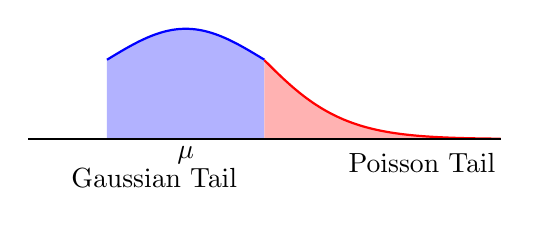
\begin{tikzpicture}
        % Plot and fill the first curve
        \fill[blue!30] (-1, 0) -- plot[domain=-1:1, smooth, variable=\x] ({\x}, {0.4 + exp(-\x*\x/2)}) -- (1, 0) -- cycle;
        \draw[domain=-1:1, smooth, variable=\x, blue, thick] plot ({\x}, {0.4 + exp(-\x*\x/2)});

        % Plot and fill the second curve, adjusting the domain and scaling for continuity
        \fill[red!30] (1, 0) -- plot[domain=1:4, smooth, variable=\x] ({\x}, {exp(-\x*ln(\x))}) -- (4, 0) -- cycle;
        \draw[domain=1:4, smooth, variable=\x, red, thick] plot ({\x}, {exp(-\x*ln(\x))});
        \draw (-2,0) -- (4,0);
        \node at (0, -0.2) {$\mu$};
        \node at (-0.4, -0.5) {Gaussian Tail};
        \node at (3, -0.3) {Poisson Tail};
    \end{tikzpicture}
\end{center}



\subsection{Applications}

\subsubsection{Mean estimation}

We start with an application of Hoeffding's inequality. Consider an i.i.d. sample \( X_1, X_2, \dots, X_n \) from $(\mu, \sigma^2)$, i.e., $\E(X_i) = \mu$ and $\var(X_i) = \sigma^2$. We want to estimate these parameters. The classical estimator of the population mean is the sample mean, i.e., $\widehat{\mu} = \dfrac{1}{n}\sum_{i=1}^n X_i$, and it turns out that $\E(\hat{\mu}) = \mu$ and hence it is unbiased, and also $\var(\hat{\mu}) = \sigma^2/n$. One can show that this is UMVUE, hence this rate of variance is optimal.

The usual confidence intervals in this case looks like $\left( \widehat{\mu} - t\sigma/\sqrt{n}, \widehat{\mu}+t\sigma/\sqrt{n} \right)$, for some $t$. However, this may not be very sharp or the best confidence interval. Because, we only get
\begin{equation*}
    \prob(\vert \hat{\mu} - \mu\vert \geq t\sigma/\sqrt{n}) \leq \dfrac{\sigma^2/n}{(t\sigma/\sqrt{n})^2} = \dfrac{1}{t^2},
\end{equation*}
\noindent by usage of Chebyshev's inequality. This is not a very sharp bound.

\textbf{Can we get sharper exponentially close to 1 confidence for general distributions? Surprisingly YES! (Note that we only assume \( \mathbb{E}|X|^2 < \infty \), not higher order moments)}.

This trick is called \textbf{Median of means} estimator. Assume $n = mK$. Partition the sample into $K$ blocks of size $m$, denoted as $B_1, B_2, \dots B_K$. Let, $\hat{\mu}_j = \dfrac{1}{m}\sum_{i \in B_j} X_i$. Define, $\tilde{\mu}$ to be the median of these blockwise means, i.e., median of $\hat{\mu}_1, \dots \hat{\mu}_K$.

The confidence interval is given in the same way as before, $\left( \tilde{\mu} - t\sigma/\sqrt{n}, \tilde{\mu}+t\sigma/\sqrt{n} \right)$, for some $t$. Note that, the error for each $\hat{\mu}_j$ is,
\begin{equation*}
    \prob\left(\hat{\mu}_j \geq \mu + \frac{t \sigma}{\sqrt{n}}\right) \leq \frac{\sigma^2/m}{(t \sigma/\sqrt{n})^2} = \frac{n/m}{t^2} = \frac{K}{t^2}
\end{equation*}
\noindent We can choose $K$ as per our convenience. Let us choose $K = t^2/4$. In this case,
\begin{equation*}
    \prob\left(\hat{\mu}_j \geq \mu + \frac{t \sigma}{\sqrt{n}}\right) \leq \frac{1}{4}.
\end{equation*}
\noindent Now, by definition of median, we have
\begin{equation*}
    \prob\left(\hat{\mu} > \mu + \frac{t \sigma}{\sqrt{n}}\right) \leq \prob\left(\text{at least } \frac{K}{2} \text{ of } \hat{\mu}_j \text{ are } \geq \frac{t \sigma}{\sqrt{n}}\right)
\end{equation*}
\noindent Note that, $Y_j = \bb{1}(\hat{\mu}_j \geq t\sigma/\sqrt{n}) \sim \text{Ber}(p)$, where $p \leq 1/4$. Let, $S_K = \frac{1}{K}\sum_{i=1}^K Y_j$. Then, $\E(S_K) = Kp \leq K/4$ and $\var(S_K) = Kp(1-p) \leq 3K/16$. Hence, applying Hoeffding's inequality, we get
\begin{align*}
    \prob\left(\hat{\mu} > \mu + \frac{t \sigma}{\sqrt{n}}\right)
     & = \prob(S_K \geq K/2)                                              \\
     & = \prob(S_K - \E(S_K) \geq K/4)                                    \\
     & \leq e^{-CK}, \text{ by Hoeffding's inequality for some large } C.
\end{align*}
\noindent Therefore, putting the value of $K$ back, we get
\begin{equation*}
    \prob\left( \vert \tilde{\mu} - \mu\vert > t\sigma/\sqrt{n} \right) \leq e^{-Ct^2/4}
\end{equation*}
\noindent Hence, the median of the means estimator provides a much narrower confidence interval for general distributions.

\subsubsection{Random Graph Phase Transition}

\begin{definitionbox}
    An Erd\"{o}s-R\'{e}nyi random graph $G(n, p)$ is a random graph consisting of $n$ nodes, and the edge between any two nodes exists with probably $p$ independent of the other edges of the graph.
\end{definitionbox}

The degree of a vertex $\text{deg}(i) = d_i = \# \text{edges connected to } i$. Clearly, $d_i \sim \text{Binom}(n-1, p)$. Therefore, $\E(d_i) = (n-1)p := d$. Turns out there is a phase transition. If $d < c\log(n)$, the random graph ends up with a giant component in between with a large probability. On the other hand, when $d > C\log(n)$, then the random graph becomes connected and regular with high probability.

\begin{figure}[h]
    \centering
    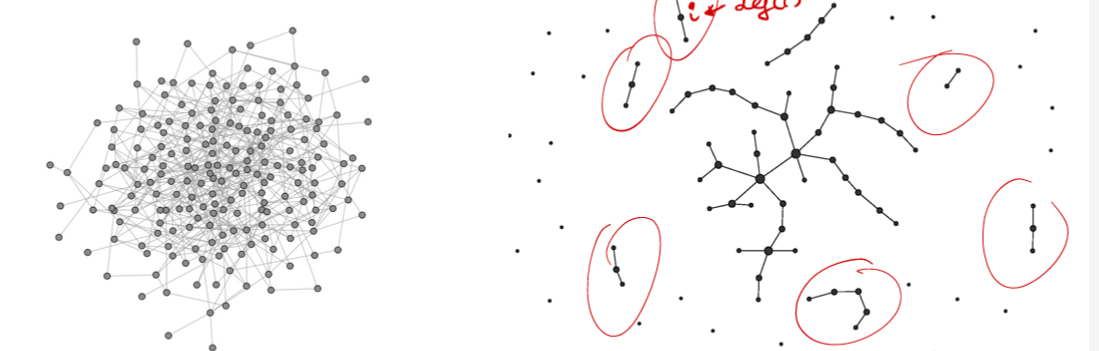
\includegraphics[width=\linewidth]{random-graph-phase-transition.png}
    \caption{Phase transitions of Erdos-Renyi random graph}
    \label{fig:random-graph-phase-transition}
\end{figure}

\begin{theorembox}
    There exists absolute constant $C > 0$, such that if $d \geq C\log(n)$, then $G(n,p)$ is almost $d$-regular with high probability. That means,
    \begin{equation*}
        \prob\left( \forall i, \text{deg}(i) : 0.9 d \leq d_i \leq 1.1 d \right) \geq 0.99
    \end{equation*}
\end{theorembox}
\begin{proof}
    Fix any $i$, let $E_i$ be the event that $\left|d_i - d\right| \leq \delta d$. Say $\delta \leq 1$. Then, by Chernoff inequality, we have
    \begin{equation*}
        \prob(E_i^c) \leq e^{-\delta^2 d/6} \leq e^{-\delta^2/6 \times C\log(n)} \leq \dfrac{1}{100n} ,
    \end{equation*}
    \noindent by choosing sufficiently large $C$. Now, union bound applies, i.e.,
    \begin{equation*}
        \prob\left( \bigcap_{i=1}^{N} E_i \right) \geq 1 - \sum_{i=1}^{n} P(E_i) \geq 1 - n\times \dfrac{1}{100n} = 0.99.
    \end{equation*}
\end{proof}

\begin{theorembox}[No regularity, but high degree clique]
    $\exists$ absolute constant $C > 0$ s.t. $d < C \log n$, the random graph $G(n, p)$ has a vertex with a large degree with high probability. These are called \textbf{hubs}. Mathematically,
    \begin{equation*}
        \prob\left( \exists i, \text{deg}(i) = d_i \geq 10d  \right) \approx 0.9.
    \end{equation*}
\end{theorembox}

\begin{proof}
    Since $d_i \sim \text{Binom}(n-1, p)$ with $\E(d_i) = d$, by application of reverse Chernoff inequality, we have
    \begin{align*}
        \prob(d_i \geq 10d)
         & \geq e^{-\mu} \left( \mu / t \right)^t, \ \text{ where } t = 10d \\
         & = e^{-d} (1/10)^{10d} \geq e^{-20d}                              \\
         & \geq e^{-20Clog(n)} \geq \dfrac{100}{n}
    \end{align*}
    \noindent by choosing sufficiently small $C$. Let, $E_i$ be the event that $d_i \geq 10d$ for any fixed $i$.

    Now if $E_i$s are independent, then it is possible that
    \begin{equation*}
        \prob\left( \cup_{i=1}^n E_i \right) = 1 - \prod_{i=1}^n \prob(E_i^c) = 1 - \left( 1 - \dfrac{100}{n} \right)^n \geq 1 - e^{-100} \geq 0.9.
    \end{equation*}
    \noindent But unfortunately, the above proof won't work since $E_i$s are not independent. Because if we have an edge between $i$ and $j$, then both $d_i$ and $d_j$ increases by one. However, for a fixed $i$ and $j$, if we ignore the edge between $i$ and $j$, the other edges of $i$ are independent of the other edges of $j$.

    So, we make some changes to the random graph $G(n, p)$ and create a new graph $G'$. In this new graph, we create two partitions of vertices, each of size $n/2$ vertices. Then we remove all the edges within the left partition, and within the right partition, but the edges remain between left and right partitions. At this point, if you pick two vertex $i$ and $j$ in the left partition, their modified degrees $\tilde{d}_i$ and $\tilde{d}_j$ are independently distributed. However, $\tilde{d}_i \sim \text{Binom}(n/2-1,p)$. It still holds that
    \begin{equation*}
        \dfrac{100}{n} \leq \prob(E_i) = \prob(d_i \geq 10d) = \prob(d_i / 2 \geq 5d) \leq \prob(\tilde{d}_i \geq 5d),
    \end{equation*}
    \noindent Now, we have
    \begin{equation*}
        \prob\left( \cup_{i=1}^n E_i \right) \geq \prob\left( \cup_{i \in \text{left half}} E_i \right) \geq 1 - \left( 1 - \dfrac{100}{n} \right)^{n/2} \geq 1 - e^{-50} \geq 0.9,
    \end{equation*}
    \noindent which completes the proof.
\end{proof}

\subsubsection{Discrepancy Theory}

Let's say we throw $N$ random points onto the 2d square $[0, 1]^2$, which are i.i.d. uniform points in $[0, 1]]^2$. Then, for all subset $I \subset [0, 1]^2$, the expected \# of points in $I$, $N_I \sim \text{Binom}(N, \lambda_I)$, where $\lambda_I$ is the area of $I$. Clearly,
\begin{align*}
    \E N_I         & = N\lambda_I                           \\
    \var(N_I)      & = N\lambda_I(1-\lambda_I) < N\lambda_I \\
    \text{sd}(N_I) & \leq \sqrt{N\lambda_I}
\end{align*}
\noindent Therefore, by Chebyshev's inequality this means, $N_I \approx N\lambda_I \pm C\sqrt{N\lambda_I}$ with high probability.

\begin{note}
    However, once the points are given, it is possible to choose a subset $I'$ such that $N_{I'} = 0$. Therefore, the above result holds only if the set is chosen predefined, and then the points are randomly distributed.
\end{note}

However, when we perform statistical methodologies, we choose the random sample first, and then analyze the data using different models. It is not that we fix the entire inference procedure beforehand, even before collecting the data. This identifies a core problem in all of statistical studies that we do currently.

This means we want some kind of result that holds regardless of the procedure used (or simultaneously for all nice classes of procedures). In the above example, it means to establish a result that is true for all nice sets $I$ simultaneously. Usually we take this class of nice sets as the convex sets, or Euclidean balls or rectangles, etc.

\begin{theorembox}
    A set of $N$ i.i.d. uniform random points on $[0, 1]^2$ satisfies the following with probability at least $0.99$ (or any $1-\epsilon$ for a given $\epsilon > 0$): For all axis-aligned rectangle $I$, we have
    \begin{equation*}
        \lambda_I N - C\sqrt{\lambda_I N \log(N)} \leq N_I \leq \lambda_I N + C\sqrt{\lambda_I N \log(N)}
    \end{equation*}
    \noindent for an absolute constant $C$ and sufficiently large $N$.
\end{theorembox}

\begin{note}
    \begin{enumerate}
        \item We lose a $\sqrt{\log(N)}$ factor to establish the uniform bound.
        \item Simple union bound may not be possible since there are infinite \# of rectangles. The idea is similar to $\epsilon$-nets and we consider $\epsilon$-grid lines and the rectangles generated by them alone.
    \end{enumerate}
\end{note}

\begin{proof}
    We use an $\epsilon$-net argument, by considering $\epsilon$-grid lines over $[0, 1]^2$ and the rectangles generated by them. We call these \textbf{net rectangles}.

    \textbf{Step 1 (Concentration):} Fix any net rectanlge $I$, with area $\lambda_I$. Then, as $N_I \sim \text{Binom}(N, \lambda_I)$, by Chernoff's inequality, we have
    \begin{align*}
                 & \prob\left( \vert N_I - \lambda_I N\vert \geq \delta \lambda_I N \right) \leq 2 e^{-\delta^2 \lambda_I N/6}                                                                            \\
        \implies & \prob\left( \vert N_I - \lambda_I N\vert \geq \lambda_I N \times C \dfrac{\sqrt{\log N}}{\sqrt{\lambda_I N}} \right) \leq 2 \exp\left[ - C^2 \log N/6 \right] \leq \dfrac{1}{N^{100}},
    \end{align*}
    \noindent for sufficiently large $C$ and $N$. Here we choose $\delta = C \dfrac{\sqrt{\log N}}{\sqrt{\lambda_I N}}$.

    \textbf{Step 2 (Union Bound):} Let $B_I$ be the event that rectangle $I$ is bad, i.e., the number of points does not fall within the required bound, i.e., $\vert N_I - \lambda_I N\vert \geq C \sqrt{\lambda_I N \log(N)}$. Now,
    \begin{equation*}
        \prob(\exists \text{ a bad } I) = \prob(\cup B_I ) \leq \sum_I \prob(B_I) \leq \left( \dfrac{1}{\epsilon} \right)^8 \dfrac{1}{N^{100}}.
    \end{equation*}
    \noindent By choosing $\epsilon = 1/N^{10}$, we have the probability that there is a bad net rectangle $I$ to be less than $\dfrac{1}{N^{20}}$, which can be made smaller than $0.99$ by choosing sufficiently large $N$.

    \textbf{Step 3 (Approximation):} This result so far holds for uniformly with high probability, but only for net rectangles. We need to show now that the number of points in any rectangle can be approximated well by the number of points in the net rectangle. Let $J$ be another rectangle, then there is a net rectangle $I$ (slightly smaller) such that
    \begin{equation*}
        \lambda_J \leq \lambda_I \leq \lambda_J + \dfrac{4}{\epsilon} = \lambda_J + \dfrac{4}{N^{10}}.
    \end{equation*}
    \noindent Therefore,
    \begin{align*}
        N_J \leq N_I
         & \leq \lambda_I N + C\sqrt{\lambda_I N \log(N)}, \ \text{ since } I \text{ is good }                                                                                     \\
         & \leq \left( \lambda_J + \dfrac{4}{N^{10}} \right)N + C\left( \left( \lambda_J + \dfrac{4}{N^{10}} \right) N \log(N) \right)^{1/2}                                       \\
         & \leq \lambda_J N + C \sqrt{\lambda_J N \log(N)} + \left( \dfrac{4}{N^9} + C \dfrac{\sqrt{4\log(N)}}{N^9} \right), \ \text{since } \sqrt{a + b} \leq \sqrt{a} + \sqrt{b} \\
         & \leq \lambda_J N + 2 C\sqrt{\lambda_J N \log(N)}, \text{ since the second term is smaller than } \sqrt{\lambda_J N \log(N)}
    \end{align*}
    \noindent This means, we only lose a factor of $2$.
\end{proof}


\subsection{Spaces of Random Variables}

\begin{definitionbox}
    A \textbf{normed space} is a vector space $M$ over field $F$ that is equipped with a norm $\norm{\cdot}$. The norm $\norm{\cdot} : M \rightarrow \R$ is a function such that
    \begin{enumerate}
        \item $\norm{x} \geq 0$ for all $x \in M$ with equality if and only if $x = 0$.
        \item $\norm{\alpha x} = \abs{\alpha}\norm{x}$ for all $\alpha \in F$ and $x \in M$.
        \item $\norm{x + y} \leq \norm{x} + \norm{y}$ for all $x, y \in M$.
    \end{enumerate}
    \noindent i.e., it has a measure of length.
\end{definitionbox}

\begin{definitionbox}
    A \textbf{Hilbert} space is a vector space $H$ over field $F$ equipped with an inner product, $\inner{\cdot,\cdot} : H \times H \rightarrow \R$ such that
    \begin{enumerate}
        \item $\inner{x, x} \geq 0$ for all $x \in H$ with equality if and only if $x = 0$.
        \item $\inner{x, y} = \inner{y, x}$ for all $x, y \in H$.
        \item $\inner{ax + by, z} = a\inner{x, z} + b\inner{y, z}$, where $a, b\in F$ and $x, y, z \in H$.
    \end{enumerate}
    \noindent i.e., it has a measure of angle, which in turn, defines length.
\end{definitionbox}

Clearly, a Hilbert space is a normed space with $\norm{x} = \sqrt{\inner{x, x}}$. We immediately have the Cacuhy-Schwartz inequality,
\begin{equation*}
    \vert \inner{x,y} \vert \leq \norm{x}\norm{y}
\end{equation*}
\noindent In case of $L^2$ space of random variables, this converts into $\vert \E(XY)\vert \leq (\E X^2)^{1/2} (\E Y^2)^{1/2}$. We also have a more general H\"{o}lder's inequality,
\begin{equation*}
    \vert \E(XY)\vert \leq \left( \E\abs{X}^p \right)^{1/p} \left( \E\abs{X}^q \right)^{1/q} = \norm{X}_{L^p} \norm{X}_{L^q},
\end{equation*}
\noindent where $(1/p + 1/q) = 1$ for some $p, q \geq 0$.

A more general is the \textbf{Jensen's} inequality, which says:
\begin{theorembox}[Jensen's inequality]
    Let $X$ be a real-valued random variable and $\phi: \R \rightarrow \R$ be a convex function. Then,
    \begin{equation*}
        \phi(\E(X)) \leq \E(\phi(X)).
    \end{equation*}
\end{theorembox}
\noindent A fact that follows from the above is that the $L^p$ norm $\norm{X}_{L^p}$ is an increasing function of $p$ for all $p \geq 1$. Before, we show the proof for this fact.

\begin{proof}
    We will show that if $p \leq q$, then $\norm{X}_{L^p} \leq \norm{X}_{L^q}$. If $p < q$, choose a function $\phi(x) = x^{q/p}$, is convex as $q > p$ or $q/p > 1$.

    By applying Jensen's inequality on this function with random variable $\abs{X}^p$,
    \begin{align*}
         & \phi(\E\abs{X}^p) \leq \E(\phi(\abs{X}^p))                \\
        \implies \left( \E\abs{X}^p \right)^{q/p} \leq \E(\abs{X}^q) \\
        \implies \norm{X}^{L^p} \leq \norm{X}_{L^q}
    \end{align*}
    \noindent where the last line follows from taking $p$-th root from both sides, and since $p \geq 1$.
\end{proof}

As a result of this, we have
\begin{equation*}
    \lim_{p \to \infty} \norm{X}_{L^p} = \norm{X}_{L^\infty} =: \text{essential supremum of } |X|.
\end{equation*}
\noindent The essential supremum is the supremum of a random variable over a set of probability $1$ discarding the set of measure zero. Also, we have,
\begin{equation*}
    L^1 \supset L^2 \supset \dots \supset L^\infty,
\end{equation*}
\noindent where $L^k$ is the space having finite $k$-th order moment and the $L^\infty$ is the space of random variables that are bounded almost surely.

\begin{note}
    Note that, $\cap_{p \geq 1} L^p \neq L^\infty$, since there are random variables (e.g. $N(0,1)$) that has finite moments for all order but still is not bounded.
\end{note}

This means, there must exists special kinds of norms that we can bound so that the resulting spaces remain in this gap. In general, we understand that $L^p$ spaces look at the $p$-th moment by considering the function $x^p$. But we could look at finite expectation of different moments like $e^x$, or $\sin(x^2)$, or something like this.

\begin{definitionbox}[Orlicz Functions]
    A function $\psi: \mathbb{R}^+ \to \mathbb{R}^+$ is called an \textbf{Orlicz function} if it is convex, increasing, and,
    \begin{equation*}
        \psi(x) \to
        \begin{cases}
            0,      & \text{as } x \to 0      \\
            \infty, & \text{as } x \to \infty
        \end{cases}
    \end{equation*}
    \noindent e.g. $\psi(x) = x^p$ or $\psi(x) = e^x - 1$.
\end{definitionbox}

\begin{definitionbox}[Orlicz norm]
    For a given Orlicz function $\psi$, the Orlicz ``norm'' of a random variable $X$ is defined as
    \begin{equation*}
        \norm{X}_{\psi} = \inf\left\{ k > 0: \E[\psi(\abs{X}/k)] \leq 1 \right\}
    \end{equation*}
\end{definitionbox}

To ensure that this definition is valid, we need to show the resulting quantity indeed defines a norm. Following is the justification for this.

\begin{enumerate}
    \item Clearly, $\norm{X}_{\psi} \geq 0$ for any random variable $X$, because it is infinimum of a set with positive quantities.
    \item If $X \equiv 0$ almost surely, then by definition of Orlicz function, $\psi(\abs{X}/k) = \psi(0) \equiv 0$ almost surely for any choice of $k > 0$. Therefore, the Orlicz norm is zero. Conversely, suppose that that Orlicz norm is $0$ but $X$ is not equal to $0$ almost surely. Then, for any $k > 0$, we must have $\E(\psi(\abs{X}/k)) \leq 1$. And since it is not true that $X$ is zero almost surely, there exists $\epsilon > 0$ such that $\abs{X} > \epsilon$ with probability at least $\delta$ for some $\delta > 0$. Also, since the Orlicz function is increasing, convex and $\psi(x) \to \infty$ as $x \to \infty$, there exists $M > 0$ such that $\psi(x) > 1/\delta$ for all $x \geq M$. Therefore, by choosing $k = \epsilon /M$, we have
          \begin{equation*}
              \E(\psi(\abs{X}/k)) = \int \psi(\abs{X}M/\epsilon)dP(x) \geq \int_{\abs{x} > \epsilon} \psi(\abs{x}M/\epsilon)dP(x) \geq \psi(M)\delta \geq 1 > 0.
          \end{equation*}
          \noindent This leads to a contradiction.
    \item The linearity of the Orlicz norm is trivial.
    \item For the triangle inequality, we need to know that for any two random variables $X$ and $Y$, $\norm{X + Y}_\psi \leq \norm{X}_\psi + \norm{Y}_\psi$. By definition of Orlicz norm, it is enough to show that for $k = \norm{X}_\psi + \norm{Y}_\psi$,
          \begin{equation*}
              \E\psi(\abs{X + Y}/k) \leq 1.
          \end{equation*}
          \noindent To see this, note that
          \begin{align*}
               & \E\psi(\abs{X + Y}/k) \\
              \leq \quad & \E\psi(\abs{X}/k + \abs{Y}/k), \text{ since } \psi \text{ is increasing } \\
              = \quad    & \E\psi\left( \dfrac{\abs{X}}{\norm{X}_\psi} \dfrac{\norm{X}_\psi}{\norm{X}_\psi + \norm{Y}_\psi} + \dfrac{\abs{Y}}{\norm{Y}_\psi} \dfrac{\norm{Y}_\psi}{\norm{X}_\psi + \norm{Y}_\psi} \right)
              = \quad    & \dfrac{\norm{X}_\psi}{\norm{X}_\psi + \norm{Y}_\psi} \E\psi\left( \dfrac{\abs{X}}{\norm{X}_\psi} \right) + \dfrac{\norm{Y}_\psi}{\norm{X}_\psi + \norm{Y}_\psi} \E\psi\left( \dfrac{\abs{Y}}{\norm{Y}_\psi} \right), \text{ since } \psi \text{ is convex } \\
              \leq \quad & \dfrac{\norm{X}_\psi}{\norm{X}_\psi + \norm{Y}_\psi} + \dfrac{\norm{Y}_\psi}{\norm{X}_\psi + \norm{Y}_\psi} = 1.
          \end{align*}
          \noindent The last inequality follows from the definition of $\norm{X}_\psi$ and $\norm{Y}_\psi$.
\end{enumerate}

Now that we know that it is indeed a well-defined norm, we can define the Orlicz space as follows.

\begin{equation*}
    L_\psi = \left\{ X: \norm{X}_\psi < \infty \right\}
\end{equation*}

To illustrate further, consider the following examples.

\begin{enumerate}
    \item If $\psi(x) = x^p$, then $\E[\psi(|X|/k)] = \E[(|X|/k)^p] \leq 1 \implies k \geq (\E[|X|^p])^{1/p}$ and $\norm{X}_\psi = \norm{X}_p$.
    \item If $\psi(x) = e^x - 1$, then $\E\psi(|X|/k) = \E[e^{|X|/k} - 1] \leq 1 \implies \E[e^{\abs{X}/k}] \leq 2$, which is something related to the MGF of a random variable.
\end{enumerate}

Now turning our attention to the Hoeffding's inequality, we note that if $X_i$s are i.i.d. symmetric Bernoulli random variables, then $\bar{X}_n = \sum_{i=1}^n X_i / n$ has Gaussian tails. The same thing holds if $X_i$ are i.i.d. standard normal random variables. Also, you can verify that if $X_i$ are i.i.d. uniform random variables on $[-1/2,1/2]$, then also $\bar{X}_n$ has Gaussian tails.

\textbf{Hence, the question is to find out the biggest class of distributions for which we have Gaussian tails.}

Turns out, if $n = 1$, then $\bar{X}_n = X_1$ needs to satisfy,
\begin{equation*}
    \prob(\abs{X_1} \geq t) \leq 2e^{-ct^2/2}, \forall t > 0.
\end{equation*}
\noindent since the above needs to be true for all choices of $n$. Therefore, this is a necessary condition. Turns out this is also sufficient for the Hoeffding lemma to hold. The random variables which has tails satisfying the above inequality are called \textbf{sub-Gaussian random variables}.


\subsubsection{Sub Gaussian Random Variables}

Before we look at the general behaviour of them, let us look at the special case for $X_i \sim N(0, 1)$. In this case,
\begin{enumerate}
    \item \textbf{Tails:} We have $\prob(|X_i| \geq t) \leq 2e^{-t^2/2}$, $\forall t > 0$.
    \item \textbf{Moments:} $\E(X_i^p) = 0$ if $p$ is odd and is equal to $(p-1)!!$ if $p$ is even. This means that the $L^p$ norm of the Gaussian random variable satisfy
          \begin{equation*}
              \norm{X_i}_p = \left( \E(\abs{X_i}^p) \right)^{1/p} \leq \left( (p-1)(p-3)\dots 5\times 3 \times 1 \right)^{1/p} \leq (p^{p/2})^{1/p} = \sqrt{p}
          \end{equation*}
          \noindent for all $p \geq 1$.
    \item \textbf{MGF:} The MGF of $X_i$ is given by $\E(e^{tX_i}) = e^{t^2/2}$.
    \item \textbf{MGF of square:} The MGF of $X_i^2$ is given by $\E(e^{tX_i^2}) = \dfrac{1}{\sqrt{1-2t}}$, if $t < 1/2$. Otherwise it is infinite. Therefore, if we take the Orlicz function $\psi_2(x) = e^{x^2} -1$, then
          \begin{align*}
                       & \E\psi(\abs{X_i}/k) \leq 1                  \\
              \implies & \E\left[ e^{X_i^2/k^2} \right] \leq 2       \\
              \implies & \dfrac{1}{\sqrt{1 - 2 \times 1/k^2}} \leq 2 \\
              implies  & k \geq \sqrt{2}.
              \implies & \norm{X_i}_{\psi_2} \leq \sqrt{2}.
          \end{align*}
\end{enumerate}

The following lemma establishes that this connection between the finiteness of all these quantities is not special for Gaussian random variables, but for all sub-Gaussian random variables.

\begin{lemma}[sub-Gaussian Lemma]
    For all random variable $X$, the following the equivalent.
    \begin{enumerate}
        \item $\exists K_1$ such that $\prob(\abs{X} \geq t) \leq 2 e^{-t^2/K_1^2}$, for all $t > 0$.
        \item $\exists K_2$ such that $\norm{X}_p \leq K_2 \sqrt{p}$, for all $p \geq 1$.
        \item $\exists K_3$ such that $\E\exp(X^2/K_3^2) \leq 2$.
        \item If $\E(X) = 0$, then $\exists K_4$ such that $\E\exp(\lambda X) \leq e^{\lambda^2 K_4^2}$, for all $\lambda \in \mathbb{R}$.
    \end{enumerate}
    \noindent These constants $K_1, \dots, K_4$, are all equivalent to the sub-Gaussian norm $\norm{X}_{\psi_2}$.
\end{lemma}

\begin{proof}
    \textbf{$(1) \implies (2)$:} Without loss of generality, assume that $K_1 = 1$. Then,
    \begin{align*}
        \E\abs{X}^p
         & = \int_{0}^\infty \prob(\abs{X}^p > t) dt                                                \\
         & = \int_{0}^\infty \prob(\abs{X} > s) p s^{p-1} ds,\  \text{ by substitution of } t = s^p \\
         & \leq \int_{0}^\infty 2e^{-s^2} ps^{p-1} ds                                               \\
         & = p(p/2 - 1)! \ \text{ as it is Gamma integral }                                         \\
         & \leq p p^{p/2 - 1} = p^{p/2}.
    \end{align*}
    \noindent Therefore, $\norm{X}_{L^p} \leq \sqrt{p}$.

    \textbf{$(2) \implies (3)$:} Without loss of generality, assume $K_2 = 1$. Then,
    \begin{align*}
        \E(e^{X^2/100})
         & = \E\left( \sum_{p=0}^\infty \dfrac{(X^2/100)^p}{p!} \right)   \\
         & = \sum_{p=0}^\infty \dfrac{1}{p! (100)^p} \E(X^{2p})           \\
         & \leq \sum_{p=0}^\infty \dfrac{1}{p! (100)^p} (2p)^{p}          \\
         & \text{ since by Stirling's approximation } p! \geq e^{-p}p^p   \\
         & \leq \sum_{p=0}^\infty \dfrac{(2p)^p}{(100)^p (p/e)^p}         \\
         & = \sum_{p=0}^{\infty} \left( \dfrac{2e}{100} \right)^p \leq 2.
    \end{align*}

    \textbf{$(3) \implies (4)$:} Without loss of generality, assume that $K_3 = 1$. We know that $e^x \leq x + e^{x^2}$ for all $x \in \R$. Therefore,
    \begin{align*}
        \E(e^{\lambda X})
         & \leq \E(\lambda X) + \E(e^{\lambda^2 X^2})                                           \\
         & = 0 + \left( \E(e^{X^2}) \right)^{\lambda^2}, \ \text{ assume } \abs{\lambda} \leq 1 \\
         & \leq 2^{\lambda^2} = e^{\lambda^2 \log(2)}.
    \end{align*}

    \textbf{$(4) \implies (1)$:} Without loss of generality, assume that $K_4 = 1$. Then,
    \begin{align*}
        \prob(\abs{X} \geq t)
         & = \prob(e^{\lambda \abs{x}} \geq e^{\lambda t})                               \\
         & \leq e^{-\lambda t} \E(e^{\lambda \abs{X}}), \ \text{ by Markov's inequality} \\
         & \leq e^{-\lambda t} e^{\lambda^2}                                             \\
         & = e^{-\lambda t + \lambda^2}
    \end{align*}
    \noindent Optimizing over $\lambda$, we get $\lambda = t/2$, yielding the bound $e^{-t^2/4}$.
\end{proof}

\begin{lemmabox}
    If $X_i$s are independent mean zero sub-Gaussian random variables, then $\norm{\sum_i X_i}_{\psi_2} \leq C \sum_{i=1}^n \norm{X_i}_{\psi_2}$ for some absolute constant $C$.
\end{lemmabox}

\begin{proof}
    We will make use of the sub-Gaussian Lemma. Note that,
    \begin{align*}
        \E(e^{\lambda \sum_i X_i})
         & = \prod_{i=1}^n \E(e^{\lambda X_i}), \ \text{ by independence } \\
         & \leq \prod_{i=1}^n e^{C \norm{X_i}_{\psi_2}^2 \lambda_i^2}      \\
         & = e^{C \sum_i \norm{X_i}_{\psi_2}^2 \lambda_i^2}.
    \end{align*}
    \noindent By equivalence of the sub-Gaussian properties, we get that $\sum_{i} X_i$ is also a sub-Gaussian random variable and that
    \begin{equation*}
        \norm{\sum_i X_i}_{\psi_2} \leq C' \sum_{i=1}^n \norm{X_i}_{\psi_2}
    \end{equation*}
    \noindent for some constant $C'$.
\end{proof}

As a result, the Hoeffding's inequality follows for sub-Gaussian random variables as well, because the tail behaviour indicates Gaussianity.

\begin{theorembox}[Hoeffding's inequality for sub-Gaussian random variables]
    If $X_i$ are independent mean zero sub-Gaussian random variables, then
    \begin{equation*}
        \prob\left(\abs{\sum_i X_i} \geq t\right) \leq 2e^{-C t^2/\sigma^2}
    \end{equation*}
    \noindent where $\sigma^2 = \sum_{i=1}^n \norm{X_i}_{\psi_2}^2$. This $\sigma^2$ is kind of a proxy for the variance.
\end{theorembox}

However, it turns out that the sub-Gaussian class is not large enough to capture all kind of random variables that we usually deal with. For example, if $X$ is sub-Gaussian, then $X^2$ is not sub-Gaussian.
\begin{equation*}
    \prob(X^2 \geq t) = \prob(\abs{X} \geq \sqrt{t}) \asymp e^{-c(\sqrt{t})^2} = e^{-ct} >> e^{-ct^2}, \ \forall t > 0.
\end{equation*}
\noindent The tail in this case is heavier than the Gaussian case, but it still decays exponentially. We call this a \textbf{sub-exponential} random variable.

\subsubsection{Sub-exponential Random Variables}

A similar lemma as before can be stated for sub-exponential random variables.

\begin{lemma}[sub-exponential Lemma]
    For all random variable $X$, the following the equivalent.
    \begin{enumerate}
        \item $\exists K_1$ such that $\prob(\abs{X} \geq t) \leq 2 e^{-t/K_1}$, for all $t > 0$.
        \item $\exists K_2$ such that $\norm{X}_{L^p} \leq K_2 p$, for all $p \geq 1$.
        \item $\exists K_3$ such that $\E\exp(\abs{X}/K_3) \leq 2$.
        \item $\exists K_4$ such that $\E\exp(\lambda X) \leq e^{\lambda^2 K_4^2}$, for all $\abs{\lambda} \leq 1/K_4$.
    \end{enumerate}
    \noindent These constants $K_1, \dots, K_4$, are all equivalent to the sub-exponential norm $\norm{X}_{\psi_1}$.
\end{lemma}

A particular thing to note that is the last bound on the MGF does not hold for all $\lambda$, because the MGF may not converge for all $\lambda$. To understand this, note that
\begin{equation*}
    \E(e^{\lambda X})= \int_0^\infty e^{\lambda x} p(x)dx \asymp \int_0^\infty e^{\lambda x}e^{-cx} dx
\end{equation*}
\noindent so the integral converges if and only if $\lambda < c$.

Clearly, Hoeffding's inequality does not hold for sub-exponential random variables in general. Since if $n = 1$, we cannot have $\prob(\abs{X} \geq t) \leq e^{-ct^2}$. However, once we accumulate multiple independent $X_i$s, we can still obtain a Gaussian tail behaviour.

\begin{theorembox}[Bernstein's inequality]
    Let $X_i$s are independent mean zero sub-exponential random variables. Then,
    \begin{equation*}
        \prob\left( \abs{\sum_{i=1}^n X_i} \geq t  \right) \leq 2\exp\left[ - C\min\left\{ \dfrac{t^2}{\sigma^2}, \dfrac{t}{K} \right\} \right]
    \end{equation*}
    \noindent where $\sigma^2 = \sum_{i=1}^n \norm{X_i}_{\psi_1}^2$ and $K = \max_{i=1}^n \norm{X_i}_{\psi_1}$.
\end{theorembox}

\subsection{Applications: Part 2}

\subsubsection{Thin Shell Phenomenon}

Consider a Gaussian random vector $g \sim N(0, I_n)$. We expect the samples from this $N(0, I_n)$ to look like the left one, but the actual picture looks like the right one in a high-dimensional space.

\begin{figure}[h]
    \centering
    \begin{tikzpicture}
        \draw (-1.5, -1.5) rectangle (1.5, 1.5);
        \node at (0.9, 0) {$0 \in \R^n$};
        \node at (0, 0) {$\circ$};
        \foreach \Point in {(0.1, 0.4), (-0.1, 0.2), (-0.2, -0.1), (-0.2, -0.4), (0.5, 0.7), (0.2, 0.2), (-0.4, -0.8), (-0.4, 0.1), (0, -0.3), (-0.7, -0.2), (0.3, -0.4)}{
                \node at \Point {\textbullet};
            }

        \draw (10, 0) circle (1.5);
        \draw[dotted] (10, 0) circle (1);
        \foreach \Point in {(10.5, 0.6), (9.7, -0.8), (10.2, -1), (9, -0.1), (9.4, 0.5)}{
                \node at \Point {\textbullet};
            }
    \end{tikzpicture}
\end{figure}


This means the samples concentrate on a thin ring close the to boundary of a the $\sqrt{n}$-ball, instead of concentrating near zero. The next theorem establishes this fact.

\begin{theorembox}
    For $g \sim N(0, I_n)$, $\prob(0.99\sqrt{n} \leq \norm{g}_2 \leq 1.01\sqrt{n}) \geq 1 - 2e^{-cn}$, for some sufficiently small but absolute constant $c$.
\end{theorembox}

\begin{proof}
    Note that,
    \begin{equation*}
        \norm{g}_2^2 - n
        = \sum_{i=1}^n (g_i^2 - 1)
        = \sum_{i=1}^n (g_i^2 - \E(g_i^2))
    \end{equation*}
    \noindent Since the above is a sum of i.i.d. terms, we can apply concentration inequalities. In particular, $g_i$ is sub-Gaussian, so $g_i^2$ is only sub-exponential, hence we need to apply Bernstein's inequality. Using that, we get
    \begin{equation*}
        \prob\left( \vert \norm{g}_2^2 - n\vert \geq 0.01n \right) \leq 2 \exp\left[ - c\min\left( \dfrac{n^2}{\sigma^2}, \dfrac{n}{K} \right) \right]
    \end{equation*}
    \noindent where
    \begin{align*}
        \sigma^2 & = \sum_{i=1}^n \norm{g_i^2 - 1}_{\psi_1} \leq nC                                            \\
        K        & = \max_{i} \norm{g_i^2 - 1}_{\psi_1} = \norm{g_1^2 - 1}_{\psi_1} (\text{ as i.i.d.}) \leq C
    \end{align*}
    \noindent Therefore, we have
    \begin{equation*}
        \prob\left( 0.99n \leq \norm{g}_2^2 - n \leq 1.01n \right) \geq 1 - 2e^{-c' n}
    \end{equation*}
    \noindent for some $c'$. Now, note that
    \begin{equation*}
        \dfrac{\norm{g}_2 - \sqrt{n}}{\sqrt{n}} = \dfrac{\norm{g}_2^2 - n}{\sqrt{n}(\norm{g}_2 + \sqrt{n})} = \dfrac{\leq 0.01n}{\geq \sqrt{n} \times \sqrt{n}} \leq 0.01n,
    \end{equation*}
    \noindent Therefore, the result follows.
\end{proof}

\subsubsection{Dimension Reduction}

Let $x_1, x_2, \dots x_N \in \R^d$ be a set of $d$-dimensional vectors. We want to reduce or translate them into $y_1, y_2, \dots y_N \in \R^n$ where $n << d$ so that the pairwise distances are approximately preserved. Turns out, to do this effectively, we can choose $n$ to be as small as $O(\log N)$. This means, for $N$ datapoints, we can effectively capture them in a $\log(N)$ dimensional vector space without losing pairwise distances. This was proved by Johnson and Linderstrass in 1984.

\begin{theorembox}[Johnson Linderstrass, 1984]
    For all $x_1, \dots x_N \in \R^d$, there exists a linear map $T: \R^d \rightarrow \R^n$ such that with $n \leq C\log(N)$ for some absolute constant $C$, we have 
    \begin{equation*}
        0.99 \norm{x_i - x_j}_2 \leq \norm{T(x_i) - T(x_j)}_2 \leq 1.01 \norm{x_i - x_j}_2,
    \end{equation*}
    \noindent for all $i, j = 1, 2, \dots N$. 
\end{theorembox}

\begin{proof}
    Choose a random map $T$ corresponding to a random matrix $1/\sqrt{n}G$ where $G$ is a random Gaussian matrix, i.e., $G_{ij} \sim N(0, 1)$. 

    Fix any $z \in \R^d$ such that $\norm{z}_2 = 1$. Then, $Gz \sim N(0, I_n)$. Therefore, by Thin-shell phenomenon, we have 
    \begin{equation*}
        \prob\left( 0.99\sqrt{n} \leq \norm{Gz}_2 \leq 1.01 \sqrt{n} \right) \geq 1 - 2e^{-cn}.
    \end{equation*}
    \noindent Now for any $i$ and $j$ such that $x_i \neq x_j$, using the above, we have 
    \begin{align*}
        & \prob\left( 0.99\sqrt{n} \leq \norm{G\dfrac{(x_i - x_j)}{ \norm{x_i - x_j}_2 } }_2 \leq 1.01 \sqrt{n} \right) \geq 1 - 2e^{-cn}\\
        \implies & \prob\left( 0.99\norm{x_i - x_j}_2 \leq \norm{T(x_i) - T(x_j)}_2 \leq 1.01 \norm{x_i - x_j}_2 \right) \geq 1 - 2e^{-cn}
    \end{align*}
    \noindent Now, an application of union bound reveals that, the probability that the above event happens for all pair of points $x_i$ and $x_j$, is at least $1 - 2N^2 e^{-cn}$. By choosing $n = 4\log(N)/c$, we get that the lower bound is at least $1 - 2/N^2$, which is positive for all $N > 2$. 

    This means, the probability that a random map will satisfy the criterion is strictly positive, hence there exists such a projection that preserves the pairwise distances approximately.
\end{proof}

\section{Combinatorial Optimization}

Combinatorial optimizations refer to the class of optimization problems that usually requires integer or natural number solutions, also sometimes restricted to have an upper bound or lower bound limit, or takes values in a finite set. Let us look at a few example problems.

\begin{example}
    Given a list of numbers $\{ a_i \}_{i=1}^n$, find the maximum possible value of $\sum_{i=1}^n a_i x_i$ subject to the restriction that $x_i \in \{ +1, -1 \}$. This is a linear objective function, and there exists a direct solution by taking $x_i = \text{sign}(a_i)$.
\end{example}

\begin{example}
    Given a list of numbers $\{ a_{ij} \}_{i,j=1}^n$, find the maximum possible value of $\sum_{i=1}^n\sum_{j=1}^n a_{ij} x_iy_j$ subject to the restriction that $x_i \in \{ +1, -1 \}, y_j \in \{ +1, -1\}$. This is a quadratic objective function. Turns out this is an NP-hard problem. Even if we restrict $x_i = y_i$, the problem still remains NP-hard.
\end{example}

Therefore, we should look at some kind of relaxation in order to be able to solve this problem efficiently. 

\begin{enumerate}
    \item \textbf{Spectral Relaxation:} Currently, we need to optimize over the boolean cube $\{-1, +1\}^n$. Instead, we can optimize this over the $\sqrt{n}$-ball $B(0, \sqrt{n})$. This allows us to algebraic manipulation to use theories of vector space. In particular, note that 
    \begin{equation*}
        \max_{x \in \{-1, +1\}^n} \sum_{i,j} a_{ij}x_i x_j \leq \max_{\norm{x} \leq \sqrt{n}} \sum_{i,j} a_{ij}x_ix_j = (\sqrt{n})^2 \max_{\norm{x} \leq 1} x\tr Ax = n \lambda_1(A)
    \end{equation*}
    \noindent and the maximizing $x$ is the eigenvector of $A$ corresponding to the largest eigenvalue. Here, we optimize an upper bound instead of the original objective function. However, using the upper bound allows us to apply Spectral theory and find a solution analytically. To get a proper solution to the boolean cube, we can then take $x_i = \text{sign}(e_{1i}(A))$, i.e., the signs of the coordinates of the first eigenvetor $e_1(A)$.
    \item \textbf{Semi-definite programming:} The other relaxation is to reparametrize the system bringing in new variables $z_{ij} = x_i x_j$ which leads to the linear objective function $\sum_{i,j}a_{ij}z_{ij}$, which is easy to solve. However, the matrix $Z$ comprising of the elements $z_{ij}$ need to satisfy a few broad conditions:
    \begin{enumerate}
        \item $Z$ is symmetric, since $z_{ij} = x_i x_j = x_j x_i = z_{ji}$.
        \item $Z_{ii} = x_i^2 = 1$, i.e., the diagonals are equal to $1$.
        \item $Z$ is positive definite.
    \end{enumerate}
    \noindent Therefore, one can consider a relaxed version of the problem with new parameter $z_{ij}$ where $Z$ satisfy the above conditions, and the objective function becomes linear. Moreover, the constraints lead to a convex set hence the entire system can be efficiently solved by using convex programming.
\end{enumerate}

\noindent Now, we present a few small applications where this kind of combinatorial optimization problem may appear.

\textbf{Ising Model:} Ising model is a model to explain electromagnetism. According to this model, every atom has a spin or polarity. When electricity is passed through the object, the polarity of the atoms of that object lines up together, and the overall magnetism property starts building up. Let $x_i$ be the state of the $i$-th atom (i.e., $+1$ or $-1$, depending on the polarity of the atom), and let $a_{ij}$ be the interaction strength between atom $i$ and atom $j$ (which is reciprocal of the squared distance between atom $i$ and atom $j$). Then, the overall energy of the system is given by the Hamiltonian,
\begin{equation*}
    H(x) = \sum_{i,j} a_{ij}x_i x_j,
\end{equation*}
\noindent which is also called free energy. Given a material, the objective is to find the maximum energy or magnetism possible.

\textbf{Clustering of Points:} Let $v_1, v_2, \dots v_n \in \R^d$ be points, and let $a_{ij} = \norm{v_i - v_j}_2$. We want to cluster these points. Let, $x_i$ be a quantity that takes values $+1$ or $-1$ depending on which cluster the point $v_i$ is in. Now, the core objective of the clustering should be, 
\begin{enumerate}
    \item If $x_ix_j = 1$, then $a_{ij}$ should be small since both $v_i$ and $v_j$ belongs to the same cluster.
    \item If $x_i x_j = -1$, then $a_{ij}$ would be large as they belong to the different clusters.
\end{enumerate}
\noindent Therefore, the objective is to minimize the objective function
\begin{multline*}
    \min_{x_i \in \{ -1, +1\}} \sum_{i,j}a_{ij}x_i x_j = \sum \text{distance in cluster 1} + \sum \text{distance in cluster 2}\\
    - \sum \text{distance between clusters}
\end{multline*}
\noindent Frieze-Jerrum (1997) generalizes the same idea for multiple clusters and solves it.

\textbf{Max-cut of a graph:} Given a graph $G = (V, E)$, the max cut problem aims to find two disjoint partitions $V_1$ and $V_2$ of the vertex set $V$ such that the \# of edges between $V_1$ and $V_2$ are largest possible. Therefore, the maximum cut objective function is
\begin{equation*}
    \textbf{Max cut of } G = \max_{V = V_1 \cup V_2} \vert E(V_1, V_2)\vert.
\end{equation*}
\noindent To solve this, consider the adjacency matrix $A$ such that $a_{ij} = \bb{1}((i, j) \in E)$. Let, $x_i = 1$ if the vertex $i$ is in $V_1$, otherwise it is $(-1)$. Therefore,
\begin{equation*}
    (1 - x_i x_j) = \begin{cases}
        2 & \text{ if } (i, j) \in E(V_1, V_2)\\
        0 & \text{ otherwise }
    \end{cases}
\end{equation*}
\noindent So, $E(V_1, V_2)$ is the number of edges between crossing over two partitions and is given by $\sum_{i,j} a_{ij}(1 - x_ix_j)/4$. 


Now that we have seen some applications where this combinatorial problem is applicable, and also seen how we can create a relaxation of this, let us try to solve the relaxed problem. We will show that in certain cases, the solution to the relaxed version is not very far from the largest value of the quadratic forms.

\begin{definitionbox}[Gram Matrix]
    The gram matrix of the vectors $v_1, v_2, \dots v_n \in \R^d$ is a $n\times n$-matrix with entries $\inner{v_i, v_j}$. 
\end{definitionbox}

\begin{lemmabox}
    For any $n \times n$ positive semi-definite matrix, there exists a choice of vectors $v_1, v_2, \dots v_n$ such that it can be written as a Gram matrix of this set of vectors.
\end{lemmabox}

\begin{proof}
    The proof follows easily from the Cholesky decomposition of the p.d. matrix.
\end{proof}

Using this lemma along with the semi-definite relaxation, we can write the matrix $Z$ as a Gram matrix, so that $z_{ij} = \inner{v_i, v_j}$. Also, we need $z_{ii} = 1 = \norm{v_i}_2^2$, i.e., the vectors $v_1, \dots v_n$ are unit vectors. Therefore, the objective becomes
\begin{equation*}
    \max_{z_{ij}} \sum_{i,j} a_{ij} z_{ij} = \max_{v_i \in \R^n, \norm{v_i} = 1} \sum_{i,j} a_{ij}\inner{v_i, v_j}
\end{equation*}
\noindent Compare this to the original combinatorial problem
\begin{equation*}
    \max_{x_i \in \{ -1, +1\} } \sum_{i,j} a_{ij}x_i x_j.
\end{equation*}
\noindent One may think of these $x_i$s as unit vectors in $\R^1$ instead of $v_i \in \R^n$.

\begin{note}
    It says that the semi-definite relaxation of the optimization problem replaces that one-dimensional vectors with $n$-dimensional vectors, (apparently that would have made things more difficult, but this is not the case here).
\end{note}

Now, given a solution to the SDP (semi-definite problem), we can get back the original $x_i$ and $x_j$ but probably clustering the original vectors $v_i$s together. Ideally, we should have a clustering of the vectors as follows. Then, we can draw a line to separate them, that accordingly we can pick $x_i$ and $x_j$. If the separation vector is $v$, then we would be looking at $x_i := \text{sign}(\inner{v, v_i})$. 

\begin{figure}[h]
    \centering
    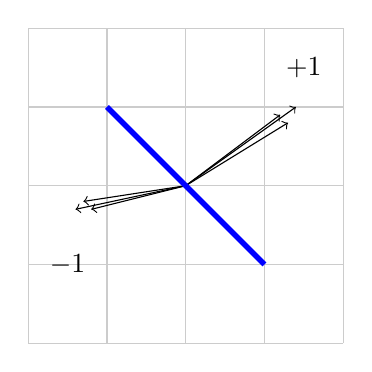
\begin{tikzpicture}
        \draw[thin,gray!40] (-2,-2) grid (2,2);
        \draw[->] (0, 0)--(1.2, 0.9);
        \draw[->] (0, 0)--(1.3, 0.8);
        \draw[->] (0, 0)--(1.4, 1);
        \draw[->] (0, 0)--(-1.2, -0.3);
        \draw[->] (0, 0)--(-1.3, -0.2);
        \draw[->] (0, 0)--(-1.4, -0.3);
        \draw[line width=2pt,blue] (-1, 1)--(1, -1);
        \node at (1.5, 1.5) {$+1$};
        \node at (-1.5, -1) {$-1$};
    \end{tikzpicture}
\end{figure}

\noindent Turns out, even a randomized cut (the algorithm is called \textbf{Randomized Rounding}), also works equally well in most cases. This means, we simply that $g \sim N(0, I_n)$, a randomly distributed Gaussian vector, and use the mapping $v \rightarrow \text{sign}(\inner{v, g})$ to get the solution.

\begin{lemmabox}[Grothendieck's identity]
    For any vectors $u, v \in \R^n$, such that $\norm{u} = \norm{v} = 1$, and a random vector $g \sim N(0, I_n)$, the following holds:
    \begin{equation*}
        \E \text{sign}(\inner{u, g})\text{sign}(\inner{v, g}) = \dfrac{2}{\pi}\sin^{-1}(\inner{u, v})
    \end{equation*}
\end{lemmabox}
\begin{proof}
    Note that, if $\theta = g/\norm{g}$, then $\theta$ is a random vector uniformly distributed on the unit $n$-dimensional hypersphere. Let $P$ be the plane on which both the vectors $u$ and $v$ reside. Since $S \cap P$ is the unit circle, $\theta$ restricted to $P$ becomes uniformly distributed on a unit circle.

    Hence, it is enough to restrict the problem to the plane $P$ since none of the inner product changes because of that. Therefore, essentially it is enough to prove the above for only $n = 2$ case.

    Let us now assume $u, v \in \R^2$ and $\theta$ is a uniformly distributed vector on the unit circle. Let's try to find out the region on the choice of $\theta$ for which we have $\text{sign}(\inner{u, \theta}) = 1$, i.e., it is the region where $\inner{u, \theta} > 0$. This means, we need to look at the perpendicular line $u^{\perp}$, and the region on the side of $u$ is this particular region where $\inner{u,\theta} > 0$. 

    \begin{figure}[h]
        \centering
        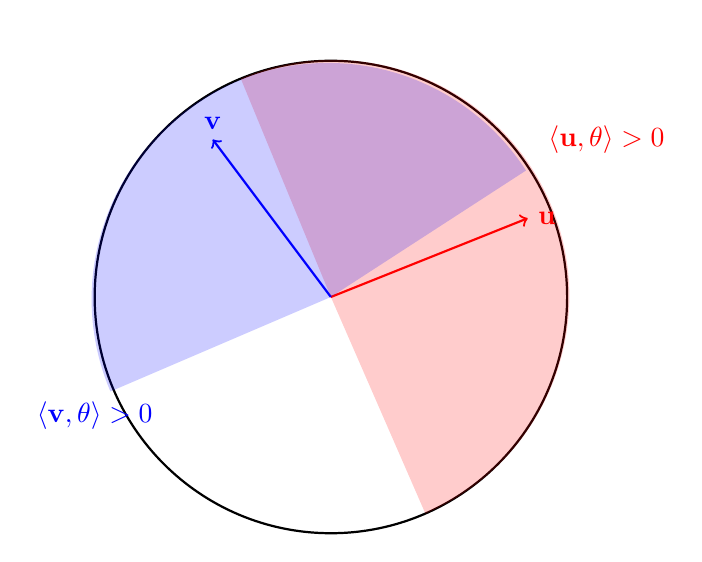
\begin{tikzpicture}
            % Draw the unit circle
            \draw[thick] (0,0) circle (3);
            
            % Draw vector u and v
            \draw[->, thick, red] (0,0) -- (2.5, 1) node[anchor=west] {$\mathbf{u}$};
            \draw[->, thick, blue] (0,0) -- (-1.5, 2) node[anchor=south] {$\mathbf{v}$};
            
            % Shaded region where <u, x> > 0
            \fill[red, opacity=0.2] (0,0) -- (1.2, -2.75) arc (-67:113:3) -- cycle;
            \node at (3.5, 2) [red] {$\langle \mathbf{u}, \mathbf{\theta} \rangle > 0$};
            
            % Shaded region where <v, x> > 0
            \fill[blue, opacity=0.2] (0,0) -- (-2.8, -1.2) arc (203:33:3) -- cycle;
            \node at (-3, -1.5) [blue] {$\langle \mathbf{v}, \mathbf{\theta} \rangle > 0$};
        \end{tikzpicture}
    \end{figure}

    By using this idea, we note that,
    \begin{equation*}
        \text{sign}(\inner{u, \theta})\text{sign}(\inner{v, \theta}) = \begin{cases}
            1 & \text{ where } \theta \in [-v^\perp, u^\perp] \cup [v^\perp, -u^\perp]\\
            (-1) & \text{ where } \theta \in [u^\perp, v^\perp] \cup [-u^\perp, -v^\perp].
        \end{cases}
    \end{equation*}
    \noindent Let, $\alpha$ be the angle between $u$ and $v$. Then,
    \begin{align*}
        \E\text{sign}(\inner{u, \theta})\text{sign}(\inner{v, \theta}) 
        & = \dfrac{1}{2\pi} \text{arclength}\left( 2 \times (2(\pi/2 - \alpha) + \alpha) - (2\pi - 2\times (2(\pi/2 - \alpha) + \alpha)) \right)\\
        & = \dfrac{1}{2\pi} \text{arclength}\left( 2\pi - 2\alpha - (2\pi - (2\pi - 2\alpha)) \right)\\
        & = \dfrac{1}{2\pi}\text{arclength}(2\pi - 4\alpha)\\
        & = 1 - \dfrac{4}{2\pi}\cos^{-1}(\inner{u, v})\\
        & = \dfrac{2}{\pi}\sin^{-1}(\inner{u, v})
    \end{align*}
\end{proof}

\begin{theorembox}[Goeman and Williamson's algorithm]
    The expected cut based on the randomized rounding partition of the solution to the SDP problem is at least $0.878$ times of the solution to the max-cut problem. 
\end{theorembox}

\begin{proof}
    The expected cut for a graph $G$ with partitions given by $x_i$s, we have 
    \begin{align*}
        \text{Expected cut} 
        & = \E\left( \dfrac{1}{4} \sum_{i,j}a_{ij}(1 - x_i x_j) \right)\\
        & = \dfrac{1}{4}\sum_{i,j}a_{ij}(1 - \E x_i x_j)\\
        & = \dfrac{1}{4}\sum_{i,j} a_{ij}(1 - \E\text{sign}(\inner{v_i, g})\text{sign}(\inner{v_j, g}))\\
        & = \dfrac{1}{4}\sum_{i,j}a_{ij}(1 - 2/\pi \sin^{-1}(\inner{v_i, v_j})), \ \text{ by Grothendieck's identity}\\
        & = \dfrac{1}{4}\sum_{i,j} a_{ij} \dfrac{2}{\pi} \cos^{-1}(\inner{v_i, v_j})\\
        & \geq \dfrac{1}{4}\sum_{i,j} a_{ij} \times 0.878 (1 - \inner{v_i, v_j}), \ \text{ by linearization of arc cosine function}\\
        & \qquad \text{ since } 2/\pi\cos^{-1}(\theta) \geq 0.878(1- \theta)\\
        & = 0.878 \times \left( \dfrac{1}{4}\sum_{i,j}a_{ij}(1 - \inner{v_i, v_j}) \right)\\
        & = 0.878 \times \text{SDP}(G) \geq 0.878 \times \text{Max cut}(G)
    \end{align*}
\end{proof}

While the above shows that the randomized rounding algorithm does not lose much in terms of tightness, one crude step we use here is that the maximum value of the SDP is at least as large as the maximum value of the original max-cut problem. The below result shows the reverse inequality up to a scaling factor to show that this relaxation is not too bad.

\begin{theorembox}[Grothendieck's inequality (1953)]
    For any $a_{ij}$ and any dimension $d$, we have
    \begin{equation*}
        \max_{u_i, v_j \in \R^d, \norm{u_i} = \norm{v_j} = 1} \sum_{i,j}a_{ij}\inner{u_i, v_j} \leq 1.782 \times \max_{x_i, y_j \in \{+1, -1\} }\sum_{i,j} a_{ij}x_i y_j
    \end{equation*}
\end{theorembox}
\begin{proof}
    The proof uses two techniques: First, a randomized rounding process. Second, a kernel trick to reach the intended nonlinearity to apply Grothendieck's lemma.

    Suppose there exists two function $\phi, \psi$ such that 
    \begin{equation*}
        \inner{\phi(u), \psi(v)} = \sin\left( \dfrac{\beta \pi}{2}\inner{u,v} \right), \ \text{ where } \beta = \dfrac{2}{\pi}\ln(1+\sqrt{2}).
    \end{equation*}
    \noindent Then by Grothendieck's identity, we have
    \begin{equation*}
        \E\text{sign}(\inner{\phi(u_i), g})\text{sign}(\inner{\psi(v_j), g}) = \dfrac{2}{\pi}\sin^{-1}\left( \inner{\phi(u_i), \psi(v_j)} \right) = \beta\inner{u_i, v_j}.
    \end{equation*}
    \noindent Therefore,
    \begin{align*}
        \sum_{i,j}a_{ij}\inner{u_i, v_j}
        & = \dfrac{1}{\beta} \sum_{i,j} a_{ij} \E\text{sign}(\inner{\phi(u_i), g})\text{sign}(\inner{\psi(v_j), g})\\
        & = \dfrac{1}{\beta} \E\left( \sum_{i,j} a_{ij}x_i^\ast y_j^\ast \right), \text{ where } x_i^\ast, y_j^\ast \in \{ -1, +1 \}\\
        & \leq \dfrac{1}{\beta} \max_{x_i, y_j \in \{-1, +1\} } \sum_{i,j} a_{ij}x_i y_j, \ \text{ and } 1/\beta = 1.782
    \end{align*}
    \noindent Taking maximum on the left-hand side now completes the solution.
\end{proof}

Now, the proof relies on the existence of $\beta, \phi$ and the $\psi$ functions. So, we will show the existence of these feature maps using tensor calculus. We shall do this in several steps.

\begin{enumerate}
    \item Let $u \in \R^n$. Then define tensor product $u \otimes u = [u_iu_j]_{i,j=1}^{n} = uu\tr \in \R^{n^2}$. Note that,
    \begin{equation*}
        \inner{u \otimes u, v\otimes v} = \sum_{i,j} u_i u_j v_i v_j = (\sum_i u_i v_i)(\sum_j u_j v_j) = \inner{u,v}^2.
    \end{equation*}
    \item Note that, similarly define $u \otimes u \otimes u$ to be the 3d-tensor with entries $u_iu_ju_k$ for all possible values of $(i,j,k)$. Similar to above, $\inner{u \otimes u\otimes u, v\otimes v \otimes v} = \inner{u,v}^3$. In general,
    \begin{equation*}
        \inner{u^{\otimes k}, v^{\otimes k}} = \inner{u, v}^k, \text{ for any } k \geq 1.
    \end{equation*}
    \item For any two vectors $u \in \R^n$ and $v \in \R^m$ ($m$ may be different from $n$), define the direct sum of them as 
    \begin{equation*}
        u \oplus v = [u_1, \dots, u_n, v_1, \dots, v_m] \in \R^{m+n}.
    \end{equation*}
    \noindent This helps us build,
    \begin{equation*}
        \inner{u \oplus v, x \oplus y} = \inner{u, x} + \inner{v, y}, \text{ provided the dimensions match}
    \end{equation*}
    \item Therefore, by combining the above two procedures (tensor product and direct sum), we can build any polynomial of the inner products. In case we want a negative coefficient, it is possible to do so by carefully choosing $\phi$ and $\psi$ to be different in one coordinate on the polynomial. For example, if we want to build $2\inner{u, v} + 3\inner{u,v}^2 - 5\inner{u, v}^3$, we take
    \begin{align*}
        \phi(u) & = \sqrt{2}u \oplus \sqrt{3}u^{\otimes 2} \oplus \sqrt{5}u^{\otimes 3} \in \R^{n + n^2 + n^3}\\
        \psi(v) & = \sqrt{2}v \oplus \sqrt{3}v^{\otimes 2} \oplus (-\sqrt{5})v^{\otimes 3} \in \R^{n + n^2 + n^3}
    \end{align*}
    \item For all real analytic function $f(x) = \sum_{k=0}^\infty c_k x^k$, we can now obtain feature maps $\phi$ and $\psi: \R^d \rightarrow L^2$ such that $\inner{\phi(u), \psi(v)} = f(\inner{u, v})$. Moreover, $\norm{\phi(u)}_2^2 = \norm{psi(v)}_2^2 = \sum_{k=0}^\infty \abs{c_k}$. For the sine function,
    \begin{align*}
        & f(x) = \sin(cx) = cx - \dfrac{(cx)^3}{3!} + \dfrac{(cx)^5}{5!} \dots \\
        \implies & \norm{\phi} = \sum_{k=0}^{\infty} = c + \dfrac{c^3}{3!} + \dfrac{c^5}{5!} + \dots = (e^c - e^{-c})/2 := 1, \ \text{ we want it to map to unit vector}\\
        \implies & c = \ln(1 + \sqrt{2}) := \dfrac{\beta \pi}{2}\\
        \implies & \beta = \dfrac{2}{\pi}\ln(1 + \sqrt{2})
    \end{align*}
\end{enumerate}

\subsection{Support Vector Machines (SVM) and Kernel Trick}

In machine learning, we use the Support Vector Machine (SVM) to perform binary classification which uses this ``kernel trick'' described above. Let's say, you have a dataset $(x_i, y_i)$ with $x_i \in \R^d$, $y_i \in \{-1, +1 \}$. We want to find a linear separation using $w \in \R^d$ such that
\begin{equation*}
    \inner{w, x_i} \begin{cases}
        > 1 & \text{ if } y_i = 1\\
        < (-1) & \text{ if } y_i = (-1)
    \end{cases}
\end{equation*}
\noindent i.e., $\inner{w, x_i} y_i > 1$ for all $i = 1, 2, \dots n$.

However, having a linear separation is overly optimistic, in practice we may not have that. Instead, we can find a feature map $\phi : \R^d \rightarrow H$ (some Hilbert space) such that on $H$, there is a linear separation. Therefore, we can find $w^\ast$ such that $\inner{w^\ast, \phi(x_i)}y_i > 1$ for all $i$. If we have $n$ datapoints, then if we have $H$ to be $n$-dimensional, we must have a linear separation. Thus, we can consider the points $x_j$s as basis, so that $w = \sum_{j} \alpha_j x_j$. With the feature map transformation, we then would have $w = \sum_j \alpha_j \phi(x_j)$. Therefore, the final objective becomes
\begin{equation*}
    \text{Find } \alpha_j \text{ such that } \sum_{j=1}^n y_j \alpha_j \inner{\phi(x_j), \phi(x_i)} > 1, \ \forall i.
\end{equation*}
\noindent Therefore, to solve this problem, one simply requires the knowledge of the inner product in the feature space, but not necessarily the feature map $H$. Hence, we can pick any positive definition function $K$ (called the kernel) and assume that
\begin{equation*}
    \inner{\phi(x_1), \phi(x_2)} := K(x_1, x_2).
\end{equation*}
\noindent This algorithm is called \textbf{Hard-margin SVM}.

Note that, hard-margin SVM perfectly classifies the binary classes, and allows no outliers. This means, even if one or two points misclassify, SVM can produce a feature map which is extremely complex. In order to allow small amount of outliers, we can combine the objectives along with a hinge-loss function.

\begin{definitionbox}[Hinge Loss]
    The hinge loss function is defined as $(1-t)_{+} = \max\{ 1 - t, 0 \}$.
\end{definitionbox}

The \textbf{Soft-margin SVM} considers the objective function to minimize
\begin{equation*}
    l(w) = \sum_{i=1}^n \left( 1 - \inner{w, x_i}y_i \right)_{+} + \lambda \norm{w}_2^2
\end{equation*}
\noindent where $\lambda$ is a penalization parameter. 

\begin{theorembox}[Mercer]
    For any continuous, symmetric and positive semi-definite kernel function $K$, there exists a map $\phi: \R^d \rightarrow H$ such that $K(x, y) = \inner{\phi(x), \phi(y)}$.
\end{theorembox}

\section{Spectral Analysis}

\subsection{Principal Component Analysis}

To visualize high-dimensional data, we use PCA (Principal Component Analysis). Let $X \in \R^d$, $\E(X) = 0$ and $\E(XX\tr) = \Sigma$. Then we can perform eigen-decomposition of $\Sigma$ to obtain the eigenvalues $\lambda_i(\Sigma)$ and the eigenvectors $v_i(\Sigma)$, which are called the ``principal components'' of $X$. 

However, we do not know $\Sigma$, we can only estimate it using a sample covariance matrix in the light of data. Given a finite sample $X_1, \dots X_n \in \R^d$, we have the estimated sample covariance matrix 
\begin{equation*}
    \Sigma_n = \dfrac{1}{n}\sum_{i=1}^n X_i X_i\tr,
\end{equation*}
\noindent assume there are mean-centered. We hope that, the PCA applied on $\Sigma_n$ will be close to PCA applied on $\Sigma$. There are two questions:

\begin{enumerate}
    \item How many samples do we require to establish this approximation?
    \item What is the error rate? 
\end{enumerate}

The answer to the first question turns out to be surprisingly only $O(d)$. That means, you need only linear many samples as the dimension to get a full picture. For the second question, we need to study some basic tools of random matrix theory.

Let's start by considering the answer to the first question. The first goal will be to show that $\Sigma_n \approx \Sigma$ in operator norm.

Let $S^{d-1}$ be the $d$-dimensional unit sphere in $\R^d$. Then,
\begin{equation*}
    \norm{\Sigma_n - \Sigma}_2^2 = \max_{v \in S^{d-1}} \abs{v\tr (\Sigma_n - \Sigma)v} = \max_{v \in S^{d-1}} \left\vert \dfrac{1}{n}\sum_{i=1}^n \inner{X_i, v}^2 - \E\inner{X, v}^2 \right\vert.
\end{equation*}
\noindent Let us call this quantity as $Z(v) = \frac{1}{n}\sum_{i=1}^n \inner{X_i, v}^2 - \E\inner{X, v}^2$. Note that, $\{ Z(v): v \in S^{d-1} \}$ is a random process indexed by $v \in S^{d-1}$. For a fixed $v$, we can show a bound by using concentration inequality. Since the maximum is taken over an uncountable set, we cannot use union bound to proceed. We need to reduce it to an $\epsilon$-net type idea.

\begin{lemmabox}
    For all $\epsilon > 0$, the sphere $S^{d-1}$ has an $\epsilon$-net $\{ x_1, x_2, \dots x_N\}$, such that $N \leq (2/\epsilon + 1)^d$.
\end{lemmabox}
\begin{proof}
    Consider the minimal $\epsilon$-net. The $\epsilon/2$-ball centered at the $x_i$s must be disjoint. If not, there exists $i \neq j$ such that $\norm{x_i - x_j} < \epsilon$, because of triangle inequality. This means, the $\epsilon$-net is not minimal since we can remove $x_j$. 

    Note that, all balls lie in the $(1 + \epsilon/2)$-ball. This means,
    \begin{align*}
        & \text{Vol}(B(1+\epsilon/2)) \geq N \text{Vol}(B(\epsilon/2))\\
        \implies & N \leq \dfrac{(1+\epsilon/2)^d}{(\epsilon/2)^d} = (2/\epsilon + 1)^d
    \end{align*}
\end{proof}
\noindent The next step in the plan is to approximate the operator norm (i.e., the maximum over $S^{d-1}$) with the maximum over an $\epsilon$-net. 

\begin{lemmabox}
    For a real symmetric matrix $A$, let $\mathcal{N} \subseteq S^{d-1}$ be an $\epsilon$-net of $S^{d-1}$, then $\norm{A} \leq 1/(1-\epsilon) \max_{x \in \mathcal{N}}\norm{Ax}$.
\end{lemmabox}
\begin{proof}
    The definition of the operator norm says that there exists $u \in S^{d-1}$ such that $\norm{Au} = \norm{A}$, since we can take $u$ to the eigenvector corresponding to the first eigenvalue of $A$ (which will have real coordinates as $A$ is real symmetric). By definition of the $\epsilon$-net, there exists $x \in \mathcal{N}$ such that $\norm{x - u} \leq \epsilon$, hence, by Cauchy-Schwartz inequality,
    \begin{equation*}
        \norm{Ax - Au} = \norm{A(x -u)} \leq \norm{A}\norm{x-u} \leq \norm{A}\epsilon.
    \end{equation*}
    \noindent Now, it follows that by triangle inequality,
    \begin{equation*}
        \norm{Ax} = \norm{Au - (Au - Ax)} \geq \norm{Au} - \norm{Ax - Au} \geq (1 - \epsilon)\norm{A}.
    \end{equation*}
    \noindent Taking maximum over all $x \in \mathcal{N}$ now completes the proof.
\end{proof}

As a corollary, if we choose $\epsilon = 1/4$, then our previous results imply that $\abs{\mathcal{N}} \leq 9^d$. Also, we get that
\begin{equation*}
    \norm{\Sigma_n - \Sigma} \leq 2 \max_{v \in \mathcal{N}} \left\vert \dfrac{1}{n}\sum_{i=1}^n \inner{X_i, v}^2 - \E\inner{X, v}^2 \right\vert.
\end{equation*}

Now, if we assume that $X_i$s are independent and subGaussian, then $\inner{X_i, v}$ is simply a linear combination of the coordinates of $X_i$, hence is also subGaussian. As a result, $\inner{X_i, v}^2$ are sub-exponential. Let $K = \norm{\inner{X_i, v}^2}_{\psi_1} = \norm{X_i\tr X_i}_{\psi_1}$ For a fixed $v \in \mathcal{N} \subseteq S^{d-1}$, using Berstein's inequality,
\begin{align*}
    \prob\left( \left\vert \dfrac{1}{n}\sum_{i=1}^n \inner{X_i, v}^2 - \E\inner{X, v}^2 \right\vert > \delta \right)
    & = \prob\left( \left\vert \sum_{i=1}^n \inner{X_i, v}^2 - \E\inner{X, v}^2 \right\vert > \delta n \right)\\
    & \leq 2 \exp\left[ - c \min\left( \dfrac{\delta^2 n^2}{K^2 n}, \dfrac{\delta n}{K} \right) \right]\\
    & = 2 \exp\left[ - c\min\left(  \dfrac{\delta^2}{K^2}, \dfrac{\delta}{K} \right)n \right]
\end{align*}

\begin{theorembox}
    If $X_i$ are independent subGaussian random variables and $n \geq Cd$ for some absolute constant $C$, then we have $\norm{\Sigma_n - \Sigma} \leq 0.1 \norm{\Sigma}$, with probability at least $1 - 2e^{-cn}$.
\end{theorembox}
\begin{proof}
    Without loss of generality, assume that $\norm{\Sigma} = 1$, otherwise, we can rescale. For a fixed $v \in S^{d-1}$, since $\norm{\Sigma} = 1$, we have
    \begin{equation*}
        \E\inner{X, v}^2 \leq \norm{\Sigma} = 1 \implies \norm{X_i}_{\psi_1} \leq C,
    \end{equation*}
    \noindent for some absolute constant $C$. Therefore, by using Berstein's inequality as shown above,
    \begin{equation*}
        \prob\left( \left\vert Z(v) \right\vert > \delta = 0.01 \right)
        \leq 2 e^{-cn}, \ \text{ for some c}.
    \end{equation*}
    \noindent By using union bound, we now have
    \begin{equation*}
        \prob\left( \max_{v \in \mathcal{N}} \left\vert Z(v) \right\vert > 0.01 \right) \leq \abs{\mathcal{N}} 2e^{-cn} = 9^d \times 2 e^{-cn} \leq 2e^{-c'n/2},
    \end{equation*}
    \noindent if $d < C"n$. This means, the complement event holds with probability $1 - 2^{-c'n/2}$, and when it holds, we have
    \begin{equation*}
        \norm{\Sigma_n - \Sigma} \leq 2 \max{v \in \mathcal{N}} \vert Z(v)\vert \leq 2 \times 0.01 \leq 0.1,
    \end{equation*}
    \noindent which completes the proof.
\end{proof}

Now that we have the ``closeness'' of $\Sigma_n$ and $\Sigma$, we want to show that the eigenvalues and the eigenvectors also remain approximately close.

\begin{theorembox}[Weyl's inequality]
    For all $d \times d$ symmetric matrices $A$ and $B$, $\max_{i} \vert \lambda_i(A) - \lambda_i(B)\vert \leq \norm{A-B}$.
\end{theorembox}
\noindent Since we have $\norm{\Sigma_n - \Sigma}$ to be small, this shows that the eigenvalues of the sample covariance matrix will closely resemble the eigenvalues of the true covariance matrix.

In the case of eigenvectors, there are some difficulties:
\begin{enumerate}
    \item Two eigenvectors may be the same up to the same sign.
    \item For a given eigenvalue with more than one geometric multiplicity, there are multiple eigenvectors that can only have a rotational invariance.
    \item Suppose two eigenvalues are close to each other, but the perturbation switches their order. Then, the corresponding eigenvectors also switch. This means, these swapped eigenvectors will be orthogonal to each other, not at all close.
\end{enumerate}
\noindent Therefore, we need to have something called a ``spectral gap'', i.e., all the eigenvalues are sufficiently apart.

\begin{theorembox}[Davis Kahan inequality]
    Let $A, B$ be two $d \times d$ symmetric matrices. Let $P_A$ be the projection operator onto the span of $\{ v_1(A), \dots, v_k(A) \}$ for some $k = 1, 2, \dots, d$. Similarly defined $P_B$ to be the projection operator onto the span of eigenvectors of $B$. Then,
    \begin{equation*}
        \norm{P_A - P_B} \leq \dfrac{\norm{A - B}}{\lambda_k(A) - \lambda_{k+1}(A)}.
    \end{equation*}
\end{theorembox}

This entire analysis now shows why the method of principal component analysis works. A few important remarks are mentioned below.

\begin{note}
    \begin{enumerate}
        \item Linear sample size $n = O(d)$ is the optimal choice in general.
        \item For structured data, it may be possible to do principal component analysis with a smaller sample size. For example, if $X = (X_1, \dots, X_1)$, then $X$ is essentially one-dimensional and then $n = O(1)$.
        \item If the data is inherently $k$-dimensional, then $n = O(k)$ is usually enough. This general result is proved by~\cite{koltchinskii2017}.
    \end{enumerate}
\end{note}

\subsection{Bulk Spectram Analysis}

\begin{figure}[h]
    \centering
    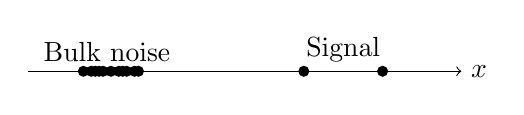
\begin{tikzpicture}
    % Draw x-axis
    \draw[->] (-0.5, 0) -- (5, 0) node[right] {$x$};
    % Points mostly grouped between 0 and 1
    \foreach \x in {0.2, 0.3, 0.35, 0.4, 0.45, 0.55, 0.65, 0.7, 0.75, 0.85, 0.9} {
        \fill (\x, 0) circle (2pt);
    }
    % Outlying points
    \fill (3, 0) circle (2pt); % Outlier at x = 3
    \fill (4, 0) circle (2pt); % Outlier at x = 4
    % Label the outliers
    \node[above] at (3.5, 0) {Signal};
    \node[above] at (0.5, 0) {Bulk noise};
    \end{tikzpicture}
    \caption{Spectral distribution of real-life data}
\end{figure}

When we analyse real-life data, we often have the above kind of picture if we plot the spectrum of the covariance matrix under consideration. Bulk of the spectrum will be distributed across a range, which consists of the noises, and then there are a few spectral values that stands out as outliers, these are only the meaningful components of the signal. Therefore, to identify the signal, we need to understand how the spectrum of pure noise would look like, as then we can remove that and get the proper signal out of the data.

The spectrum behaviour of the pure noise data is given by ``Marchenko Pastur Law (1967)''. We shall talk about this in a short while.

\subsubsection{Wigner's Law}

We begin by considering a simpler model instead. Let $W$ be a symmetric $n \times n$ random matrix such that all of its entries on and above the diagonal are i.i.d. standard normal random variables. Then Wigner's law demonstrates the asymptotic behaviour of the spectral density of $W/\sqrt{n}$. 

\begin{theorembox}[Wigner's Law (1958)]
    For the above random matrix $W$, for any $-2 \leq a \leq b \leq 2$, the number of eigenvalues of $W/\sqrt{n}$ lying between $[a, b]$, say denoted by $N_{W/\sqrt{n}}([a, b])$ satisfy
    \begin{equation*}
        \lim_{n\rightarrow \infty} \dfrac{N_{W/\sqrt{n}}([a, b])}{n} = \int_a^b \rho_{sc}(x) dx,
    \end{equation*}
    \noindent where $\rho_{sc}(x) = \sqrt{4-x^2}/2\pi$ where $x \in [-2, 2]$. This is often called the ``semicircle'' density.
\end{theorembox}

Before we aim to prove this, we need a few tools at our disposal.

\begin{enumerate}
    \item If we have a partition matrix 
    \begin{equation*}
        M = \begin{bmatrix}
            a & b\tr \\
            b & D
        \end{bmatrix},
    \end{equation*}
    \noindent then if $D$ is invertible, then the formula for Schur's complement formula says
    \begin{equation*}
        M_{11}^{-1} = \text{(1,1)-th entry of } M^{-1} = \dfrac{1}{a - b\tr D^{-1}b}.
    \end{equation*}
    \item If $g \sim N(0, I_n)$, then $\E(g\tr M g) = \trace{M}$.
    \item For a symmetric matrix $M$, we have 
    \begin{equation*}
        \lambda_i(M^{-1}) = \dfrac{1}{\lambda_i(M)}, \text{ and, } 
        \lambda_i(M - zI) = \lambda_i(M) - z, \ z \in \R.
    \end{equation*}
    \item One function that contains information about eigenvalues is $f(z) = \det(A - zI)$, for which the roots of this function are the eigenvalues.
    \item Consider another function where the eigenvalues are the poles of the function. Hence,
    \begin{equation*}
        f(z) = \dfrac{1}{n}\sum_{i=1}^n \dfrac{1}{\lambda_i - z} = \dfrac{1}{n}\sum_{i=1}^n \lambda_i( (A-zI)^{-1} ) = \dfrac{1}{n}\trace{(A - zI)^{-1}}.
    \end{equation*}
    \noindent This last matrix $(A - zI)^{-1}$ is often called ``resolvent function'' of the matrix $A$.
    \item On a similar note, one can define \textbf{Stieljes transform}. Stieljes transform of a distribution of a random variable $X$ is 
    \begin{equation*}
        S(z) = \E\left[ \dfrac{1}{X - z} \right], z \in \C.
    \end{equation*}
    \noindent It is possible to show that $S(z)$ can uniquely define the distribution of $X$ (much like the characteristic function). In fact, its inversion formula is given by
    \begin{equation*}
        f(x) = \lim_{\epsilon \rightarrow 0+} \dfrac{S(x+i\epsilon) - S(x-i\epsilon)}{2\pi i}.
    \end{equation*}
\end{enumerate}

The following is an informal proof of Wigner's law based on these ideas.

\begin{proof}
    
    
    \noindent\textbf{Step 1:} 
    Let $\lambda_1, \dots, \lambda_n$ be the eigenvalues of $W/\sqrt{n}$. Define the Stieljes transform of the empirical spectral density, 
    \begin{equation*}
        S_n(z) = \dfrac{1}{n}\sum_{i=1}^n \dfrac{1}{\lambda_i - z} = \dfrac{1}{n}\trace{\left( \dfrac{1}{\sqrt{n}}W - zI \right)^{-1}} = \dfrac{1}{n}\sum_{i=1}^n M_{ii}^{-1},
    \end{equation*}
    \noindent where $M$ is equal to the matrix $(W/\sqrt{n} - zI)$. Note that, $M$ can be partitioned as
    \begin{equation*}
        M = \begin{bmatrix}
            \dfrac{W_{11}}{\sqrt{n}} - z & \dfrac{1}{\sqrt{n}}g\tr\\
            \dfrac{1}{\sqrt{n}}g & \bar{M}\\
        \end{bmatrix},
    \end{equation*}
    \noindent where $g \sim N(0, I_{n-1})$. Therefore, by the formula of Schur's complement, we have
    \begin{align*}
        M_{11}^{-1} 
        & = \dfrac{1}{\dfrac{W_{11}}{\sqrt{n}} - z - \dfrac{1}{n}g\tr \bar{M}^{-1}g }\\
        & \approx \dfrac{1}{ 0 - z - \dfrac{1}{n}\E(g\tr \bar{M}^{-1} g) }\\
        & = \dfrac{1}{-z - \dfrac{1}{n} \trace{(\bar{M})^{-1}} }\\
        & \approx \dfrac{1}{-z - \dfrac{n}{n-1}S_{n-1}(z)}, \ \text{ assuming } \bar{M} \approx M, \text{ but just of dimension } (n-1)
    \end{align*}
    \noindent As $n \rightarrow \infty$, we have in the limit,
    \begin{equation*}
        S_\infty(z) = \lim_{n\rightarrow \infty} \dfrac{1}{n}\sum_{i=1}M_{ii}^{-1}
        = -\dfrac{1}{z + S_\infty(z)},
    \end{equation*}
    \noindent i.e., $S_\infty(z) + (z + S_\infty(z))^{-1} = 0$. Solving for $S_\infty(z)$ yields
    \begin{equation*}
        S_\infty(z) = \dfrac{-z + \sqrt{z^2 - 4}}{2}.
    \end{equation*}

    \noindent\textbf{Step 2:}
    Due to the Stieljes inversion, it is now enough to show that the semicircle distribution $\rho_{sc}(x)$ has the same Stieljes transformation.

    To see this, we note that
    \begin{align*}
        S_{sc}(z) 
        & = \dfrac{1}{2\pi} \int_{-2}^2 \dfrac{\sqrt{4 - x^2}}{x - z}dx\\
        & = \dfrac{1}{2\pi} \int_{\pi}^0 \dfrac{-4\sin^2(\theta)}{2\cos(\theta) - z} d\theta, \ \text{ letting } x = \cos(\theta)\\
        & = \dfrac{1}{\pi} \int_0^\pi \dfrac{2\sin^2(\theta)}{2\cos(\theta) - z}d\theta\\
        & = -\dfrac{1}{4i\pi} \int_{\norm{\alpha} = 1} \dfrac{(\alpha^2 - 1)^2}{\alpha^2 (\alpha^2 + 1 - \alpha z)}d\alpha, \ \text{ letting } \alpha = e^{i\theta}
    \end{align*}
    \noindent Now in the last integral, we need to apply Cauchy's Residue formula. Note that, the given function has 3 poles, at $\alpha_0 = 0$ of order $2$, at $\alpha_1 = (z+\sqrt{z^2-4})/2$ and at $\alpha_2 = (z-\sqrt{z^2-4})/2$. 

    The pole at $\alpha_1 = (z + \sqrt{z^2-4})/2$ lies outside the unit circle, hence to use the Residue theorem, we calculate the residues at $\alpha_0$ and $\alpha_2$. 
    \begin{align*}
        \text{Res}(\alpha_0)
        & = \dfrac{4\alpha_0(\alpha_0^2 - 1)(\alpha_0^2 + 1 - z\alpha_0) - (\alpha_0^2 - 1)^2(2\alpha_0 - z)}{(\alpha^2_0 + 1 - z\alpha_0)^2} = z\\
        \text{Res}(\alpha_2)
        & = \dfrac{(\alpha_2^2 - 1)^2}{\alpha_2^2 (\alpha_2 - (z + \sqrt{z^2 -4})/2)} = -\sqrt{z^2-4}
    \end{align*}
    \noindent Therefore, by applying the Residue theorem for integrals,
    \begin{equation*}
        S_{sc}(z) = -\dfrac{1}{4\pi i} \int_{\norm{\alpha} = 1} \dfrac{(\alpha^2 - 1)^2}{\alpha^2 (\alpha^2 + 1 - \alpha z)}
        = -\dfrac{2\pi i}{4\pi i} \left[ \text{Res}(\alpha_0) + \text{Res}(\alpha_2) \right] = \dfrac{-z+\sqrt{z^2 - 4}}{2},
    \end{equation*}
    \noindent which matches with the Stieljes transform $S_\infty(z)$ derived earlier.

    \noindent\textbf{Step 3:} Now we apply the Steiljes inverse to complete the proof.
\end{proof}

We have a similar theorem for the singular values which may arise from a matrix with different dimensions. 

\begin{theorembox}[Marchenko-Pastur, 1967]
    Let $X_1, X_2, \dots, X_n \sim N(0, I_d)$ and $\Sigma_n = n^{-1}\sum_{i=1}^n X_i X_i\tr$, the sample covariance matrix. Suppose that $d/n \rightarrow r \in (0, 1)$ as $n \rightarrow \infty$. Then, the spectral density of $\Sigma_n$ converges to the Marchenko Pastur law, given by
    \begin{equation*}
        \rho_{MP}(x) = \dfrac{1}{2\pi rx} \sqrt{(x-a)(b-x)}, \ x \in [a, b],
    \end{equation*}
    \noindent where $a = (1 - \sqrt{r})^2$ and $b = (1 + \sqrt{r})^2$.
\end{theorembox}

To prove this result, we need to know the following two results.

\begin{enumerate}
    \item \textbf{Stieljes transformation of MP law:} Using similar calculation as above, we can calculate the Stieljes transformation of the Marchenko Pastur law as 
    \begin{equation*}
        S_{MP}(z) = \dfrac{1 - z - r + \sqrt{(1-z-r)^2 - 4zr}}{2}.
    \end{equation*}
    \item \textbf{Sherman-Morrison Formula:} Given two vectors $x, y \in \R^d$ and $M \in \R^{d\times d}$, we have
    \begin{equation*}
        (M + xy\tr)^{-1} = M^{-1} - \dfrac{M^{-1} xy\tr M^{-1}}{1 + y\tr M^{-1}x}.
    \end{equation*}
    \noindent Let $q = y\tr M^{-1}x$. Then, we get that
    \begin{equation*}
        y\tr (M + xy\tr)^{-1}x 
        = q - \dfrac{q^2}{1 + q} = 1 - \dfrac{1}{1+q}
        = 1 - \dfrac{1}{y\tr M^{-1}x}.
    \end{equation*}
\end{enumerate}

The following is again an informal proof of Marchenko-Pastur theorem using these two basic ideas.

\begin{proof}
    Our steps will be similar to the Wigner's theorem. We shall derive the limiting Stieljes transform of the spectral density of $\Sigma_n$ and show that it matches with the Stieljes transform of MP law. Let $S_n(z)$ be the Stieljes transform of the spectral density of $\Sigma_n$, i.e.,
    \begin{equation*}
        S_n(z) 
        = \dfrac{1}{d}\sum_{k=1}^d \lambda_k(\Sigma_n - zI)^{-1}
        = \dfrac{n}{d}\trace{ \left(\sum_{i=1}^n X_i X_i\tr - nzI\right)^{-1} }
        \rightarrow \dfrac{1}{r}\trace{A^{-1}},
    \end{equation*}
    \noindent where $A$ is the matrix it is replacing, i.e., $A = \sum_{i=1}^n X_i X_i\tr - nzI$. Let $B = \sum_{i=1}^{n-1} X_i X_i\tr - nzI = A - X_nX_n\tr$. Now, it follows that

    \begin{align*}
        & X_n\tr A^{-1}X_n = X_n\tr (B + X_nX_n\tr)^{-1}X_n = 1 - \dfrac{1}{1 + X_n\tr B^{-1} X_n} \\
        \implies & X_n\tr A^{-1}X_n \approx 1 - \dfrac{1}{1 + \E(X_n\tr B^{-1}X_n ) }\\
        \implies & X_n\tr A^{-1}X_n \approx 1 - \dfrac{1}{1 + \trace{B^{-1}}}, \ \text{ since } X_n \text{ are } B \text{ independent }\\
        \implies & X_n\tr A^{-1}X_n \approx 1 - \dfrac{1}{1 +  rS_{n-1}(nz/(n-1)) } \\
        \implies & \sum_{k=1}^n X_k\tr A^{-1}X_k \approx n \left[ 1 - \dfrac{1}{1 +  rS_{n-1}(nz/(n-1)) } \right]\\
        \implies & \trace{\sum_{k=1}^n X_kX_k\tr  A^{-1}} \approx n \left[ 1 - \dfrac{1}{1 +  rS_{n-1}(nz/(n-1)) } \right]\\
        \implies & \trace{(A + nzI)A^{-1}} \approx n \left[ 1 - \dfrac{1}{1 +  rS_{n-1}(nz/(n-1)) } \right]\\
        \implies & d + nzr S_n(z) = d (1 + zS_n(z)) \approx n \left[ 1 - \dfrac{1}{1 +  rS_{n-1}(nz/(n-1)) } \right]
    \end{align*}
    \noindent Taking limit on both sides and using $S_{\infty}(z)$ to denote the limiting Stieljes transform, we obtain the relation
    \begin{equation*}
        1 + z S_\infty(z) = \dfrac{1}{r}\left[ 1 - \dfrac{1}{1 + rS_\infty(z)} \right] = \dfrac{S_\infty(z)}{1 + rS_\infty(z)}.
    \end{equation*}
    \noindent Solving this yields,
    \begin{equation*}
        S_\infty(z) = \dfrac{1 - z - r + \sqrt{(1 - z - r)^2 - 4zr} }{2}.
    \end{equation*}
\end{proof}




\pagebreak


\begin{thebibliography}{99}
    \bibitem[Koltchinskii~and~Lounici~(2017)]{koltchinskii2017} Koltchinskii, Vladimir, and Karim Lounici. "Concentration inequalities and moment bounds for sample covariance operators." Bernoulli (2017): 110-133.
\end{thebibliography}


\end{document}

